\section{Task 1: Newton--Cotes quadrature}

\subsection{Method overview and problem}
Composite Newton--Cotes quadrature integrates functions using the Newton--Cotes formula over composite intervals. It aims to improve integration precision, particularly for more complex functions.
\textbf{Assumptions:}
\begin{itemize}
    \item Function \( f \): the function to integrate.
    \item Endpoints \( a \) and \( b \): integration limits.
    \item Point count \( n \): number of interpolation points.
    \item Interval count \( m \): number of subintervals.
\end{itemize}
\textbf{Formula:}
\[
\int_a^b f(x)dx \approx \frac{b-a}{mn} \sum_{k=0}^n B_k \sum_{s=0}^{m-1} f(a + \frac{(ns + k)(b-a)}{mn})
\]
The coefficients \( B_k \) are computed using Lagrange basis polynomials.
\textbf{Key properties:}
\begin{itemize}
    \item Multiple subintervals \( m \) reduce the Runge phenomenon.
    \item Higher accuracy than simple Newton--Cotes formulas at the same point count.
    \item Applicable to both uniformly and nonuniformly continuous functions.
\end{itemize}
\subsubsection{Detailed explanation of the formula}
The method computes an integral using polynomial approximation. We fix the polynomial degree ($m$), then evaluate each integral $\int_a^b P_i$, where $P_i$ is the polynomial on subinterval $i$. Computing the integral on subinterval $i$ requires $m$ points, so the full approximation needs $n * m$ points; I did not account for this here, which is my mistake. To find $P_i$, we use Lagrange interpolation and integrate those polynomials. I did not implement a function for this either, although integrating polynomials is not difficult.


\subsection{Tests}

Tests validated the method and analyzed its errors. They included integrating \( x^2 \) over \([-1, 6]\) and comparing the result with the analytical solution.
\textbf{Error analysis:}
\begin{itemize}
    \item We compared performance for two test functions:
    \begin{itemize}
        \item Uniformly continuous function: \( \sin(x) + \cos^2(x) - x^2 + 7x \)
        \item Nonuniformly continuous function: \( \frac{1}{1+x^2} \)
    \end{itemize}
\end{itemize}
For each function we examined:
\begin{itemize}
    \item Relative and absolute errors with identical parameter settings.
    \item Parameter ranges:
    \begin{itemize}
        \item \( m \): from 1 to 4, the number of subintervals.
        \item \( n \): from 2 to 42, the number of points.
    \end{itemize}
\end{itemize}

{\centering
\paragraph{Error growth}
\indent

\paragraph{Uniformly continuous function}
\indent

\begin{minipage}{0.48\textwidth}
    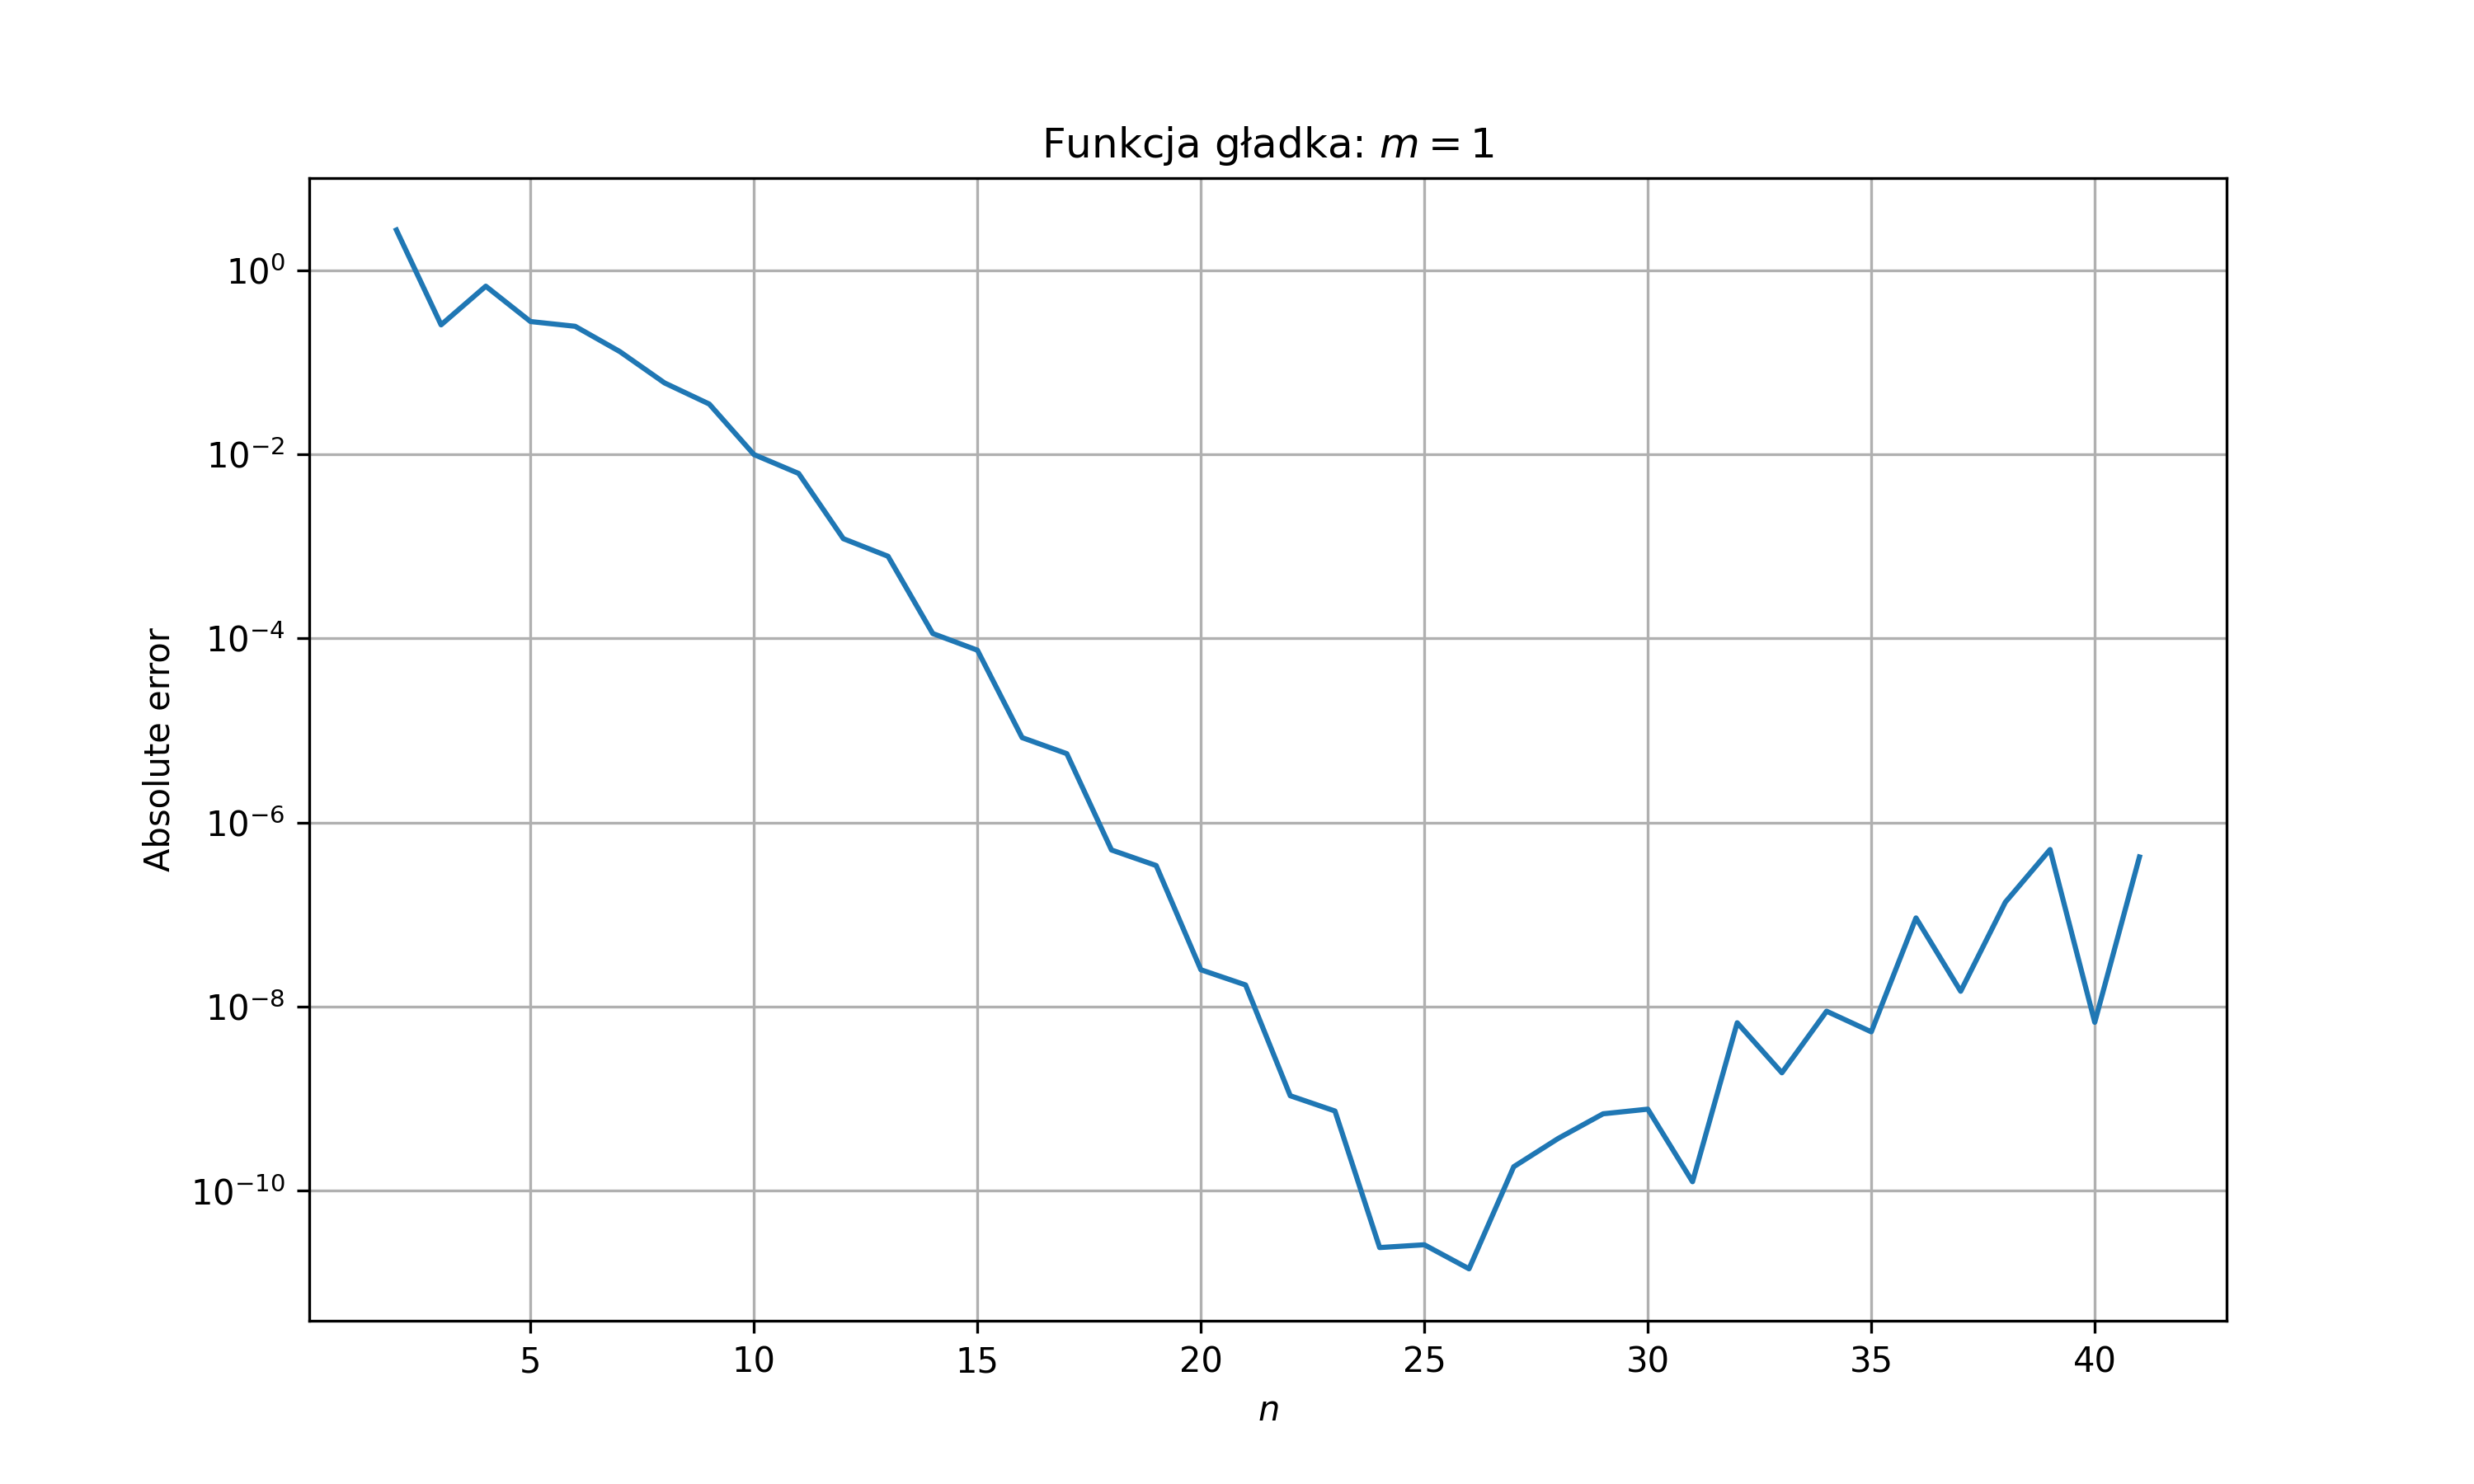
\includegraphics[width = \textwidth]{figures/task-1/abs_smth_1.png}
\end{minipage}
\begin{minipage}{0.48\textwidth}
    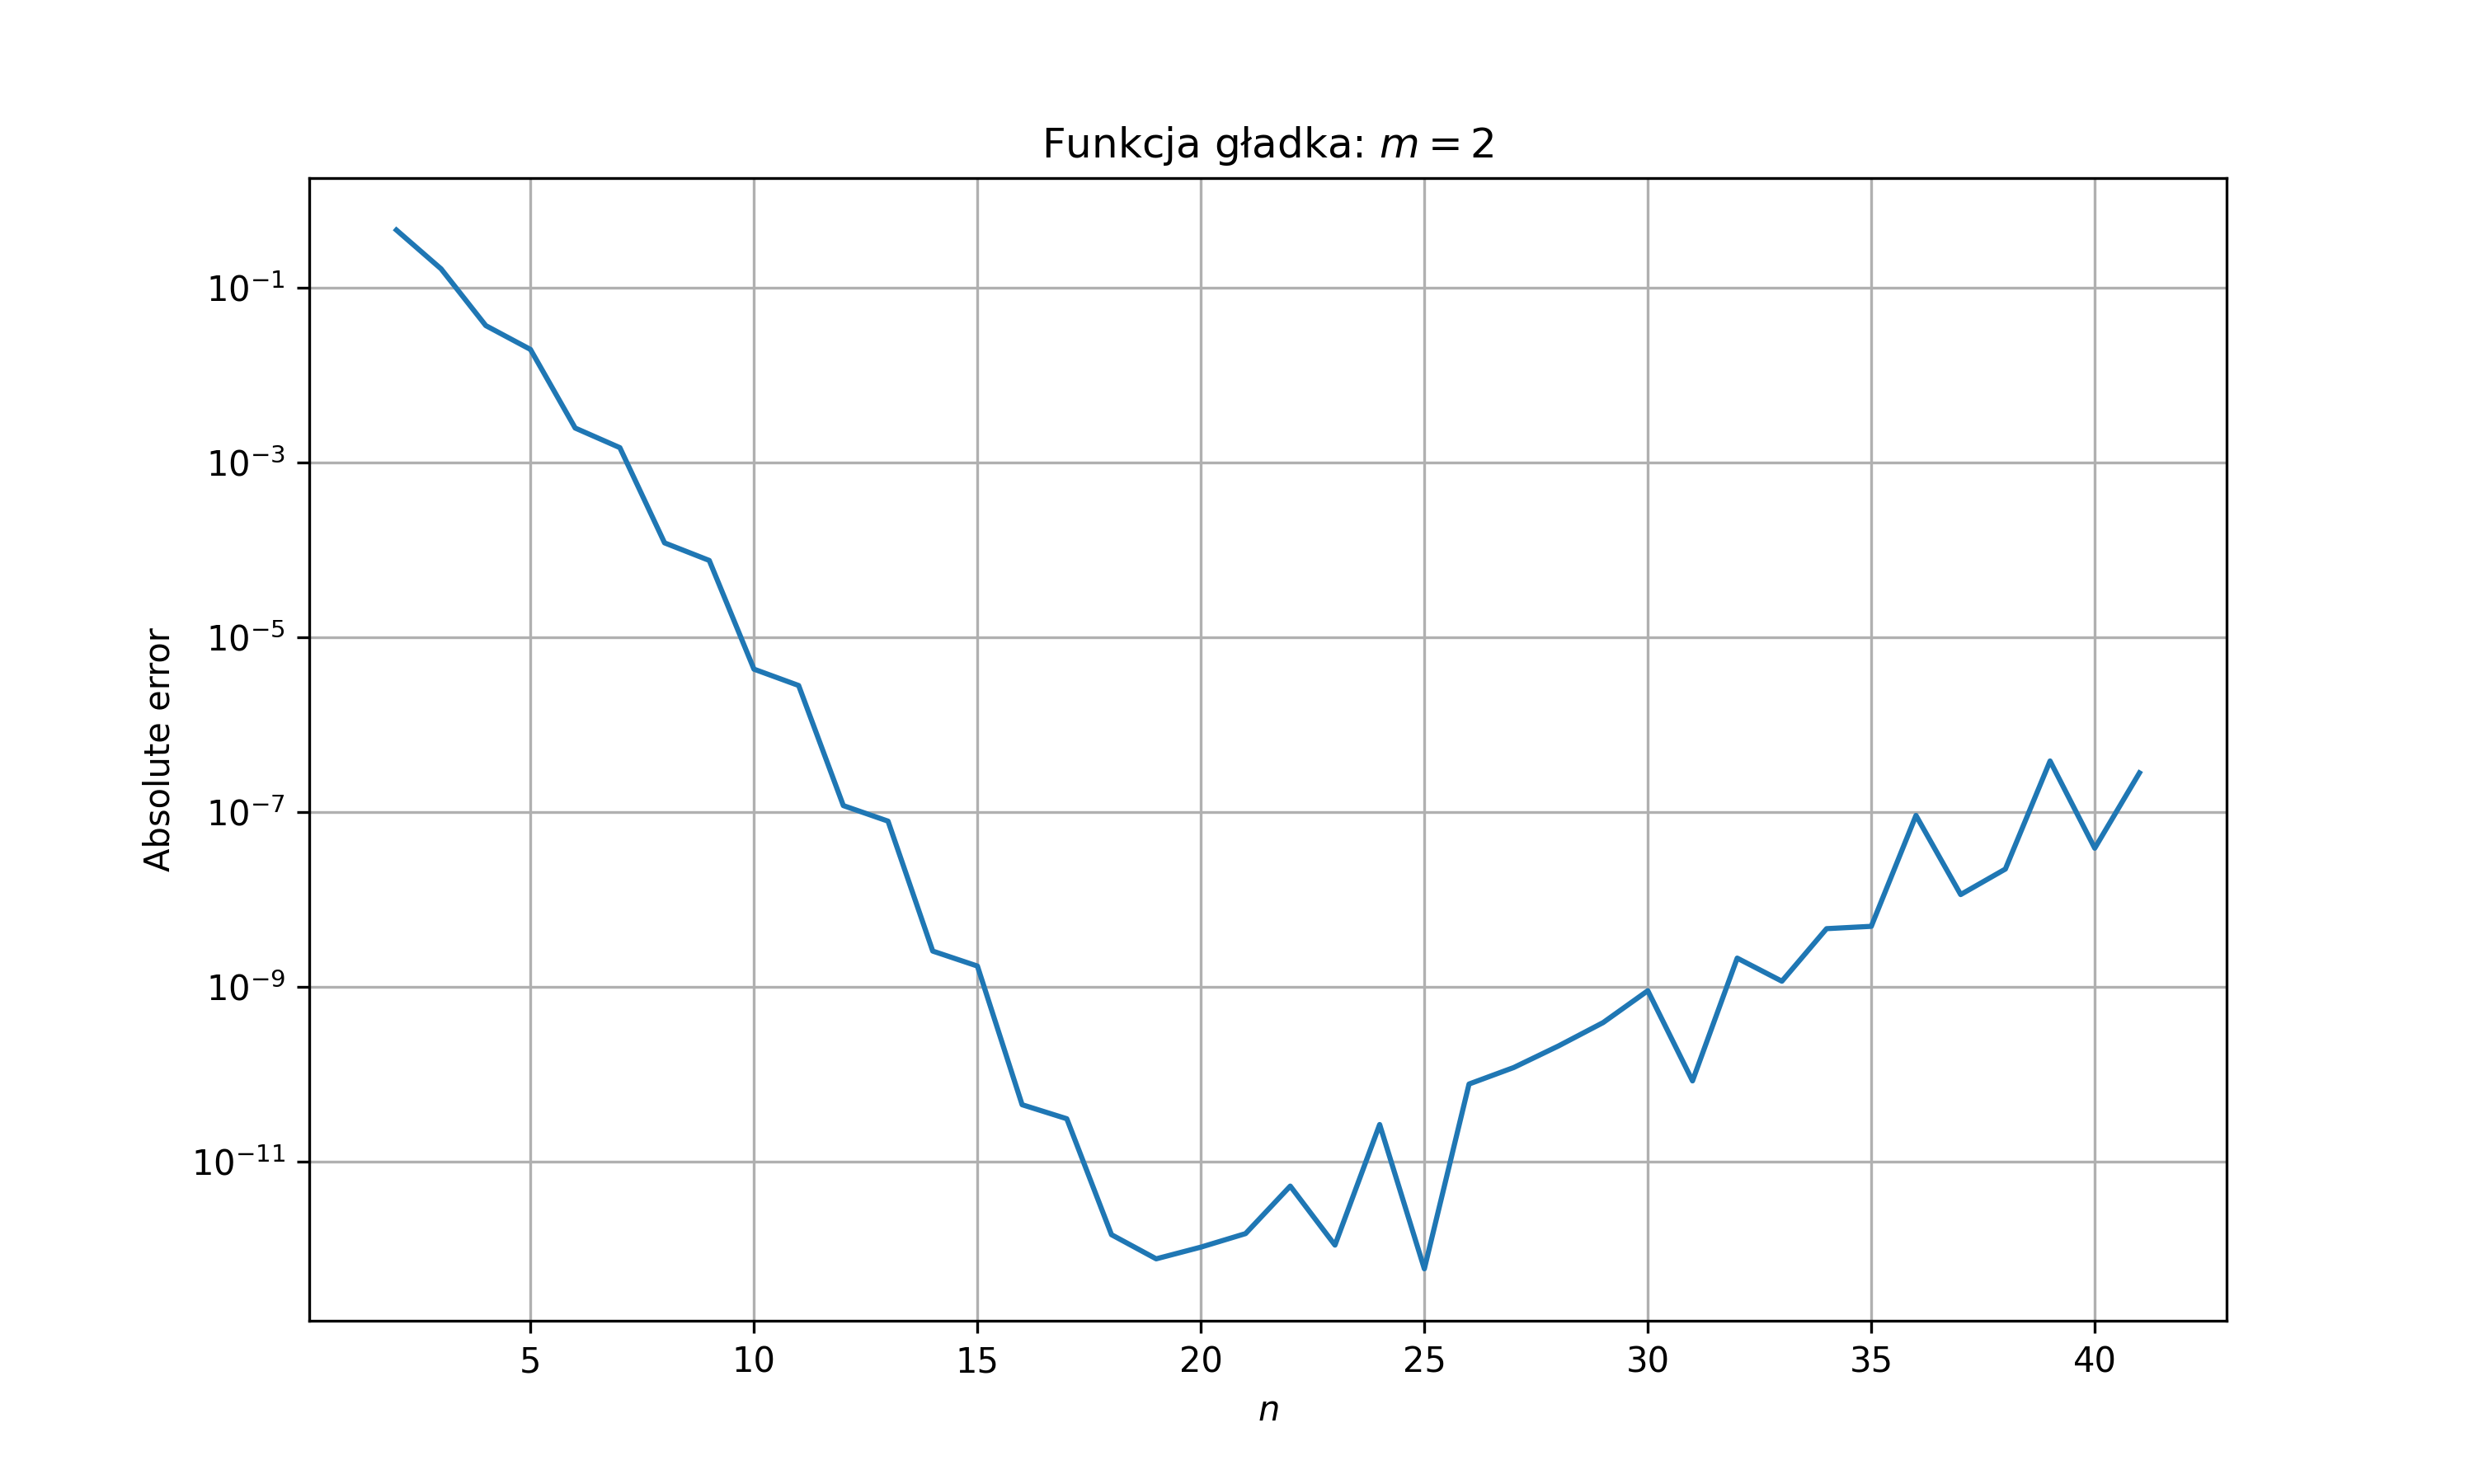
\includegraphics[width = \textwidth]{figures/task-1/abs_smth_2.png}
\end{minipage}

\begin{minipage}{0.48\textwidth}
    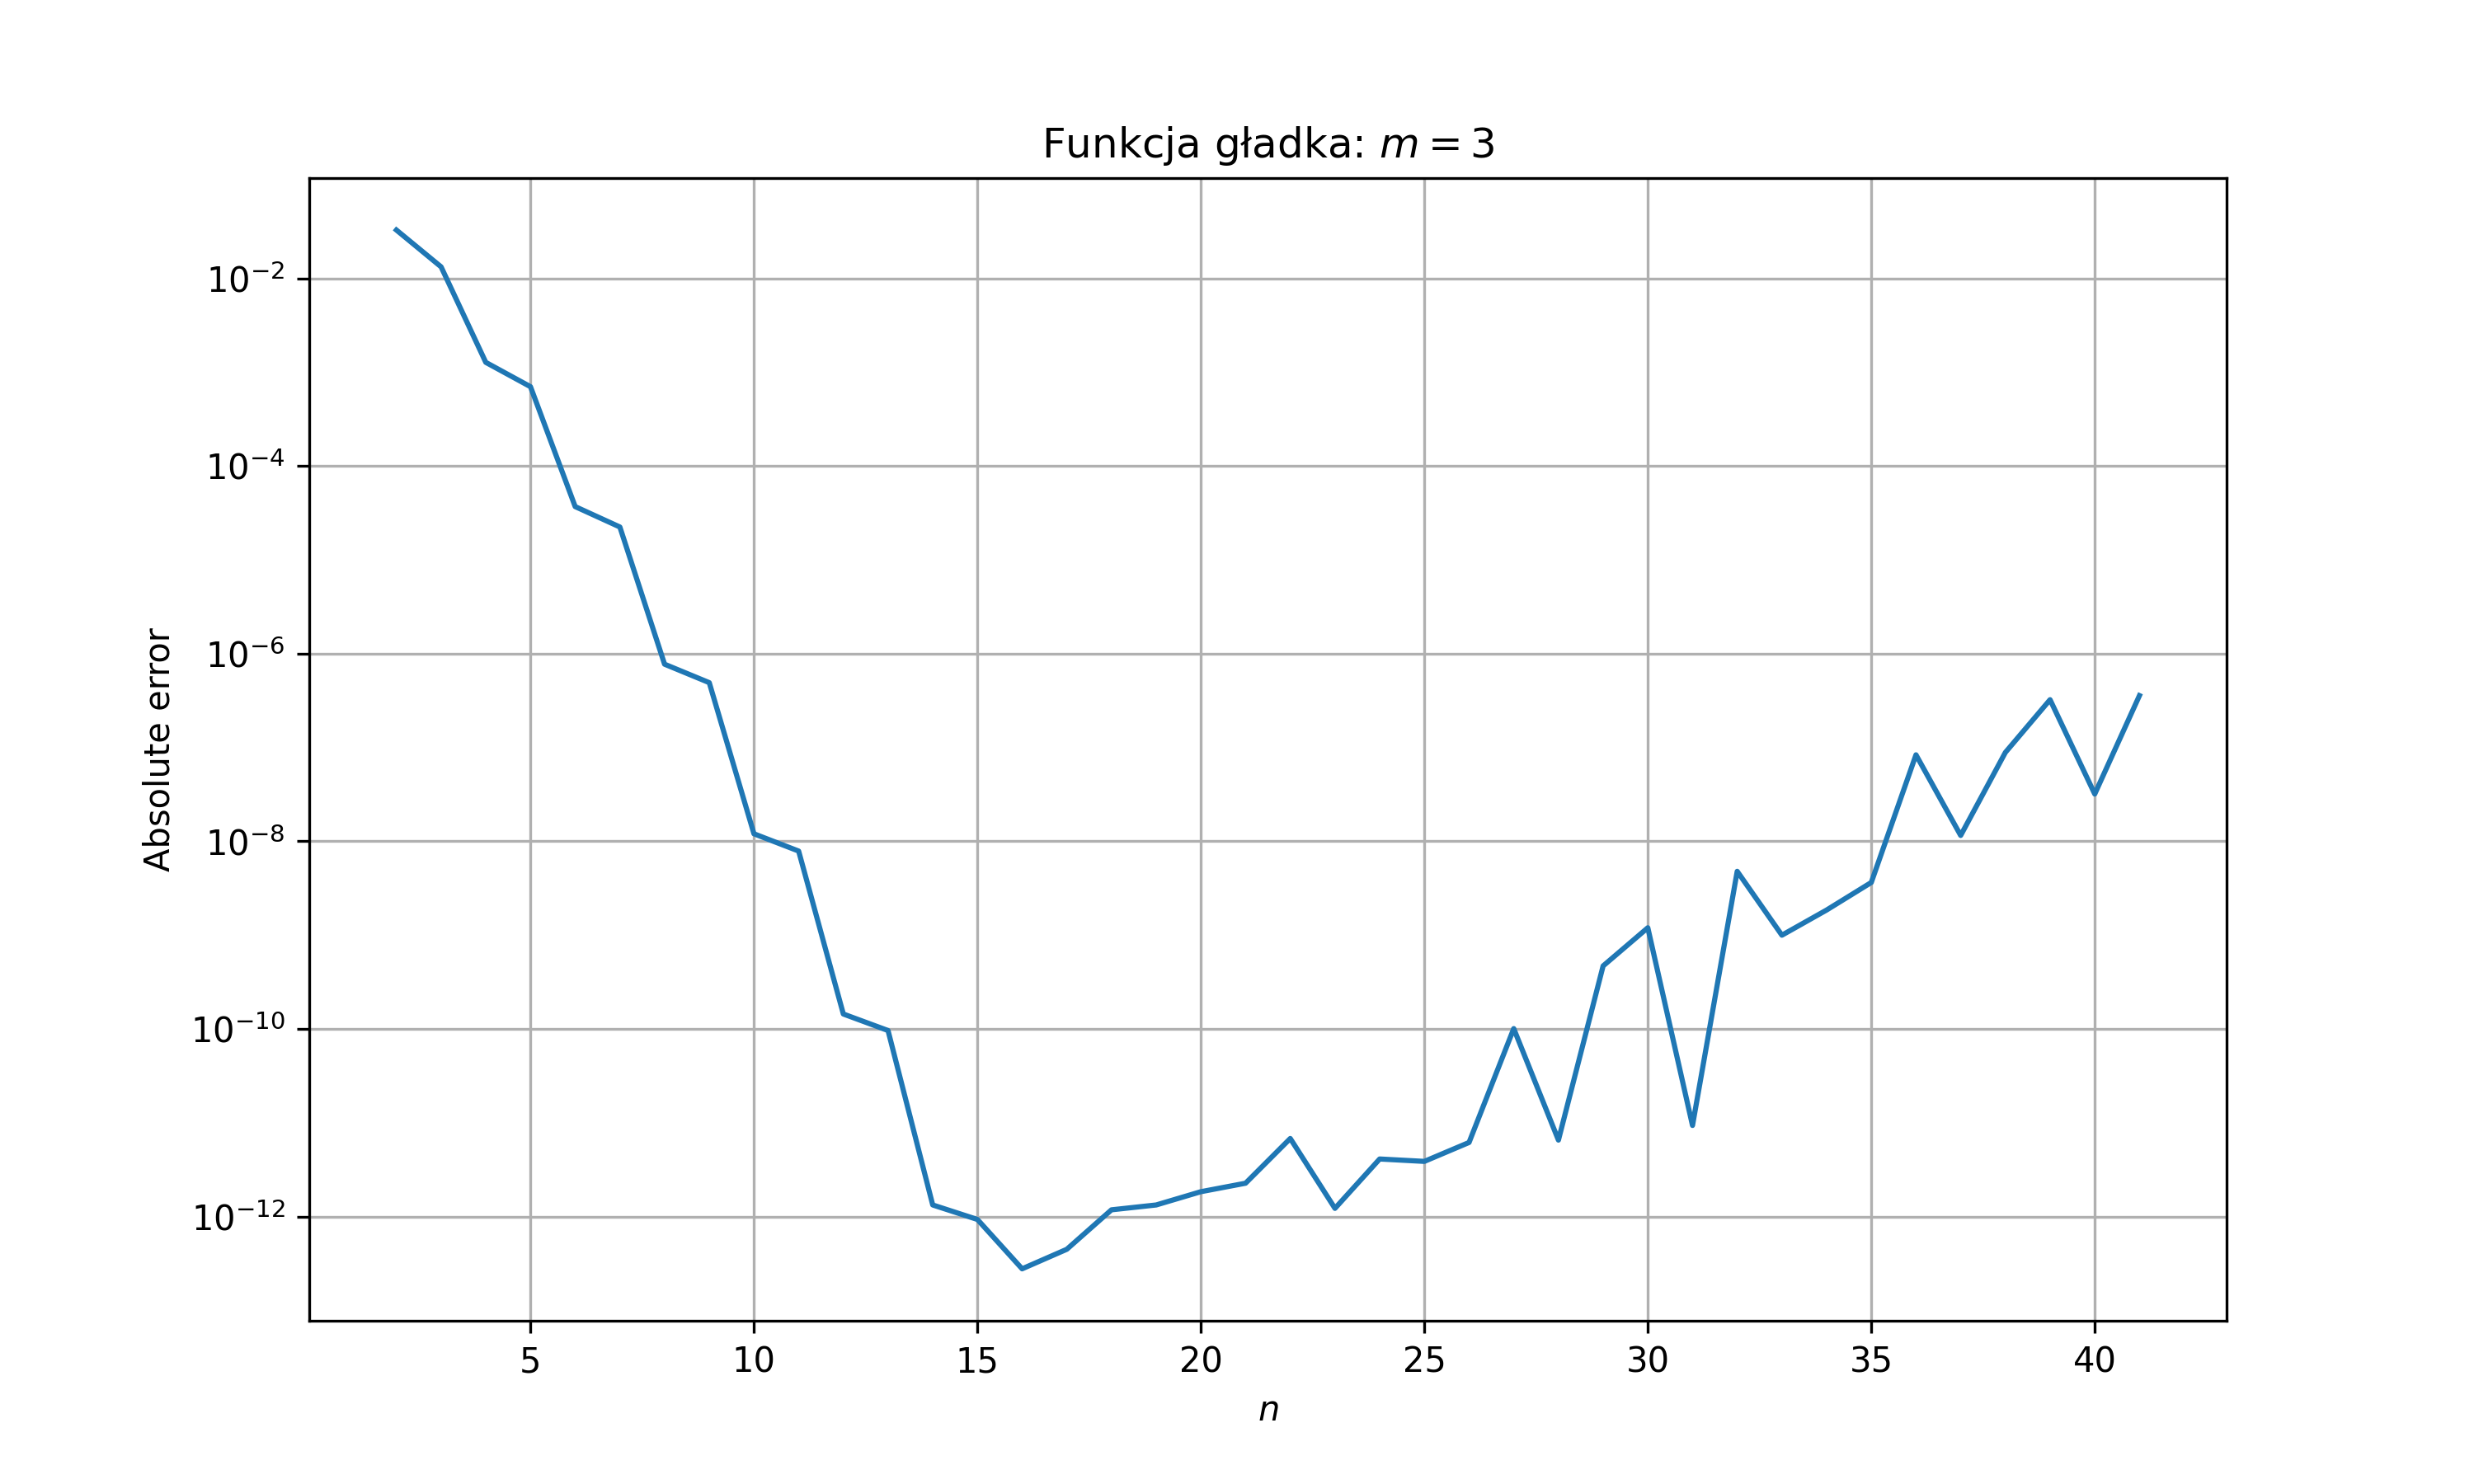
\includegraphics[width = \textwidth]{figures/task-1/abs_smth_3.png}
\end{minipage}
\begin{minipage}{0.48\textwidth}
    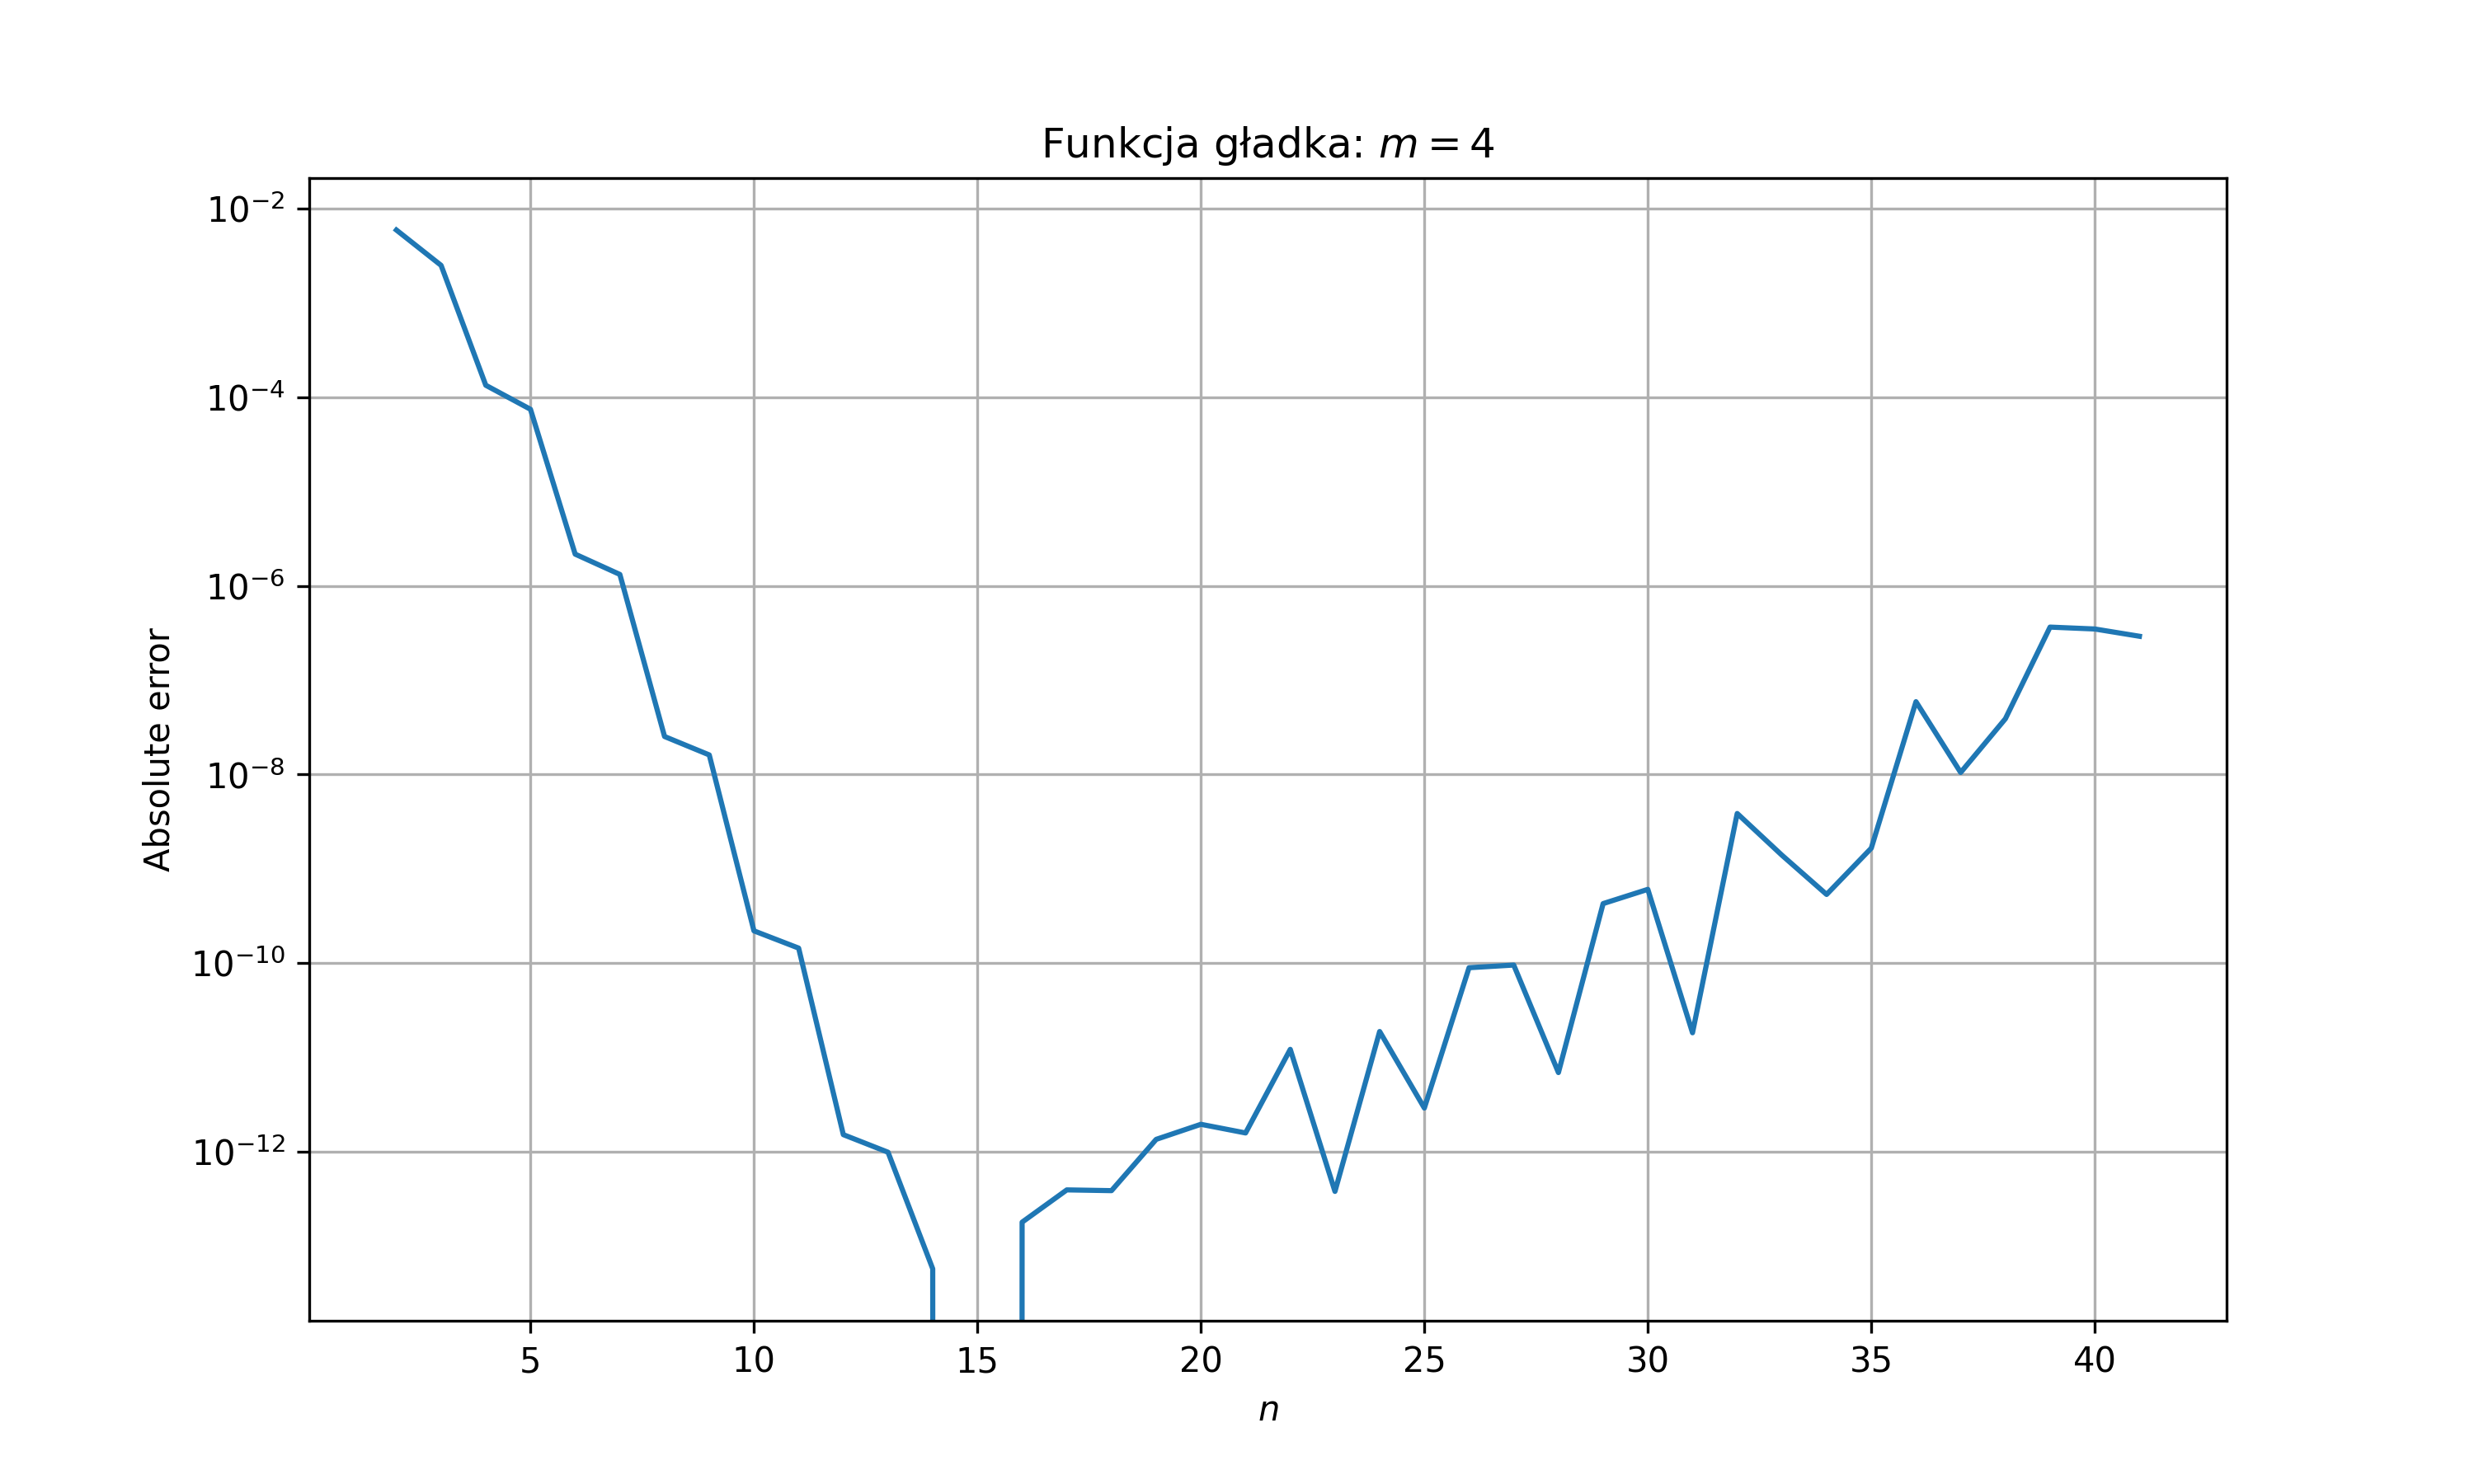
\includegraphics[width = \textwidth]{figures/task-1/abs_smth_4.png}
\end{minipage}
Relative error

\begin{minipage}{0.48\textwidth}
    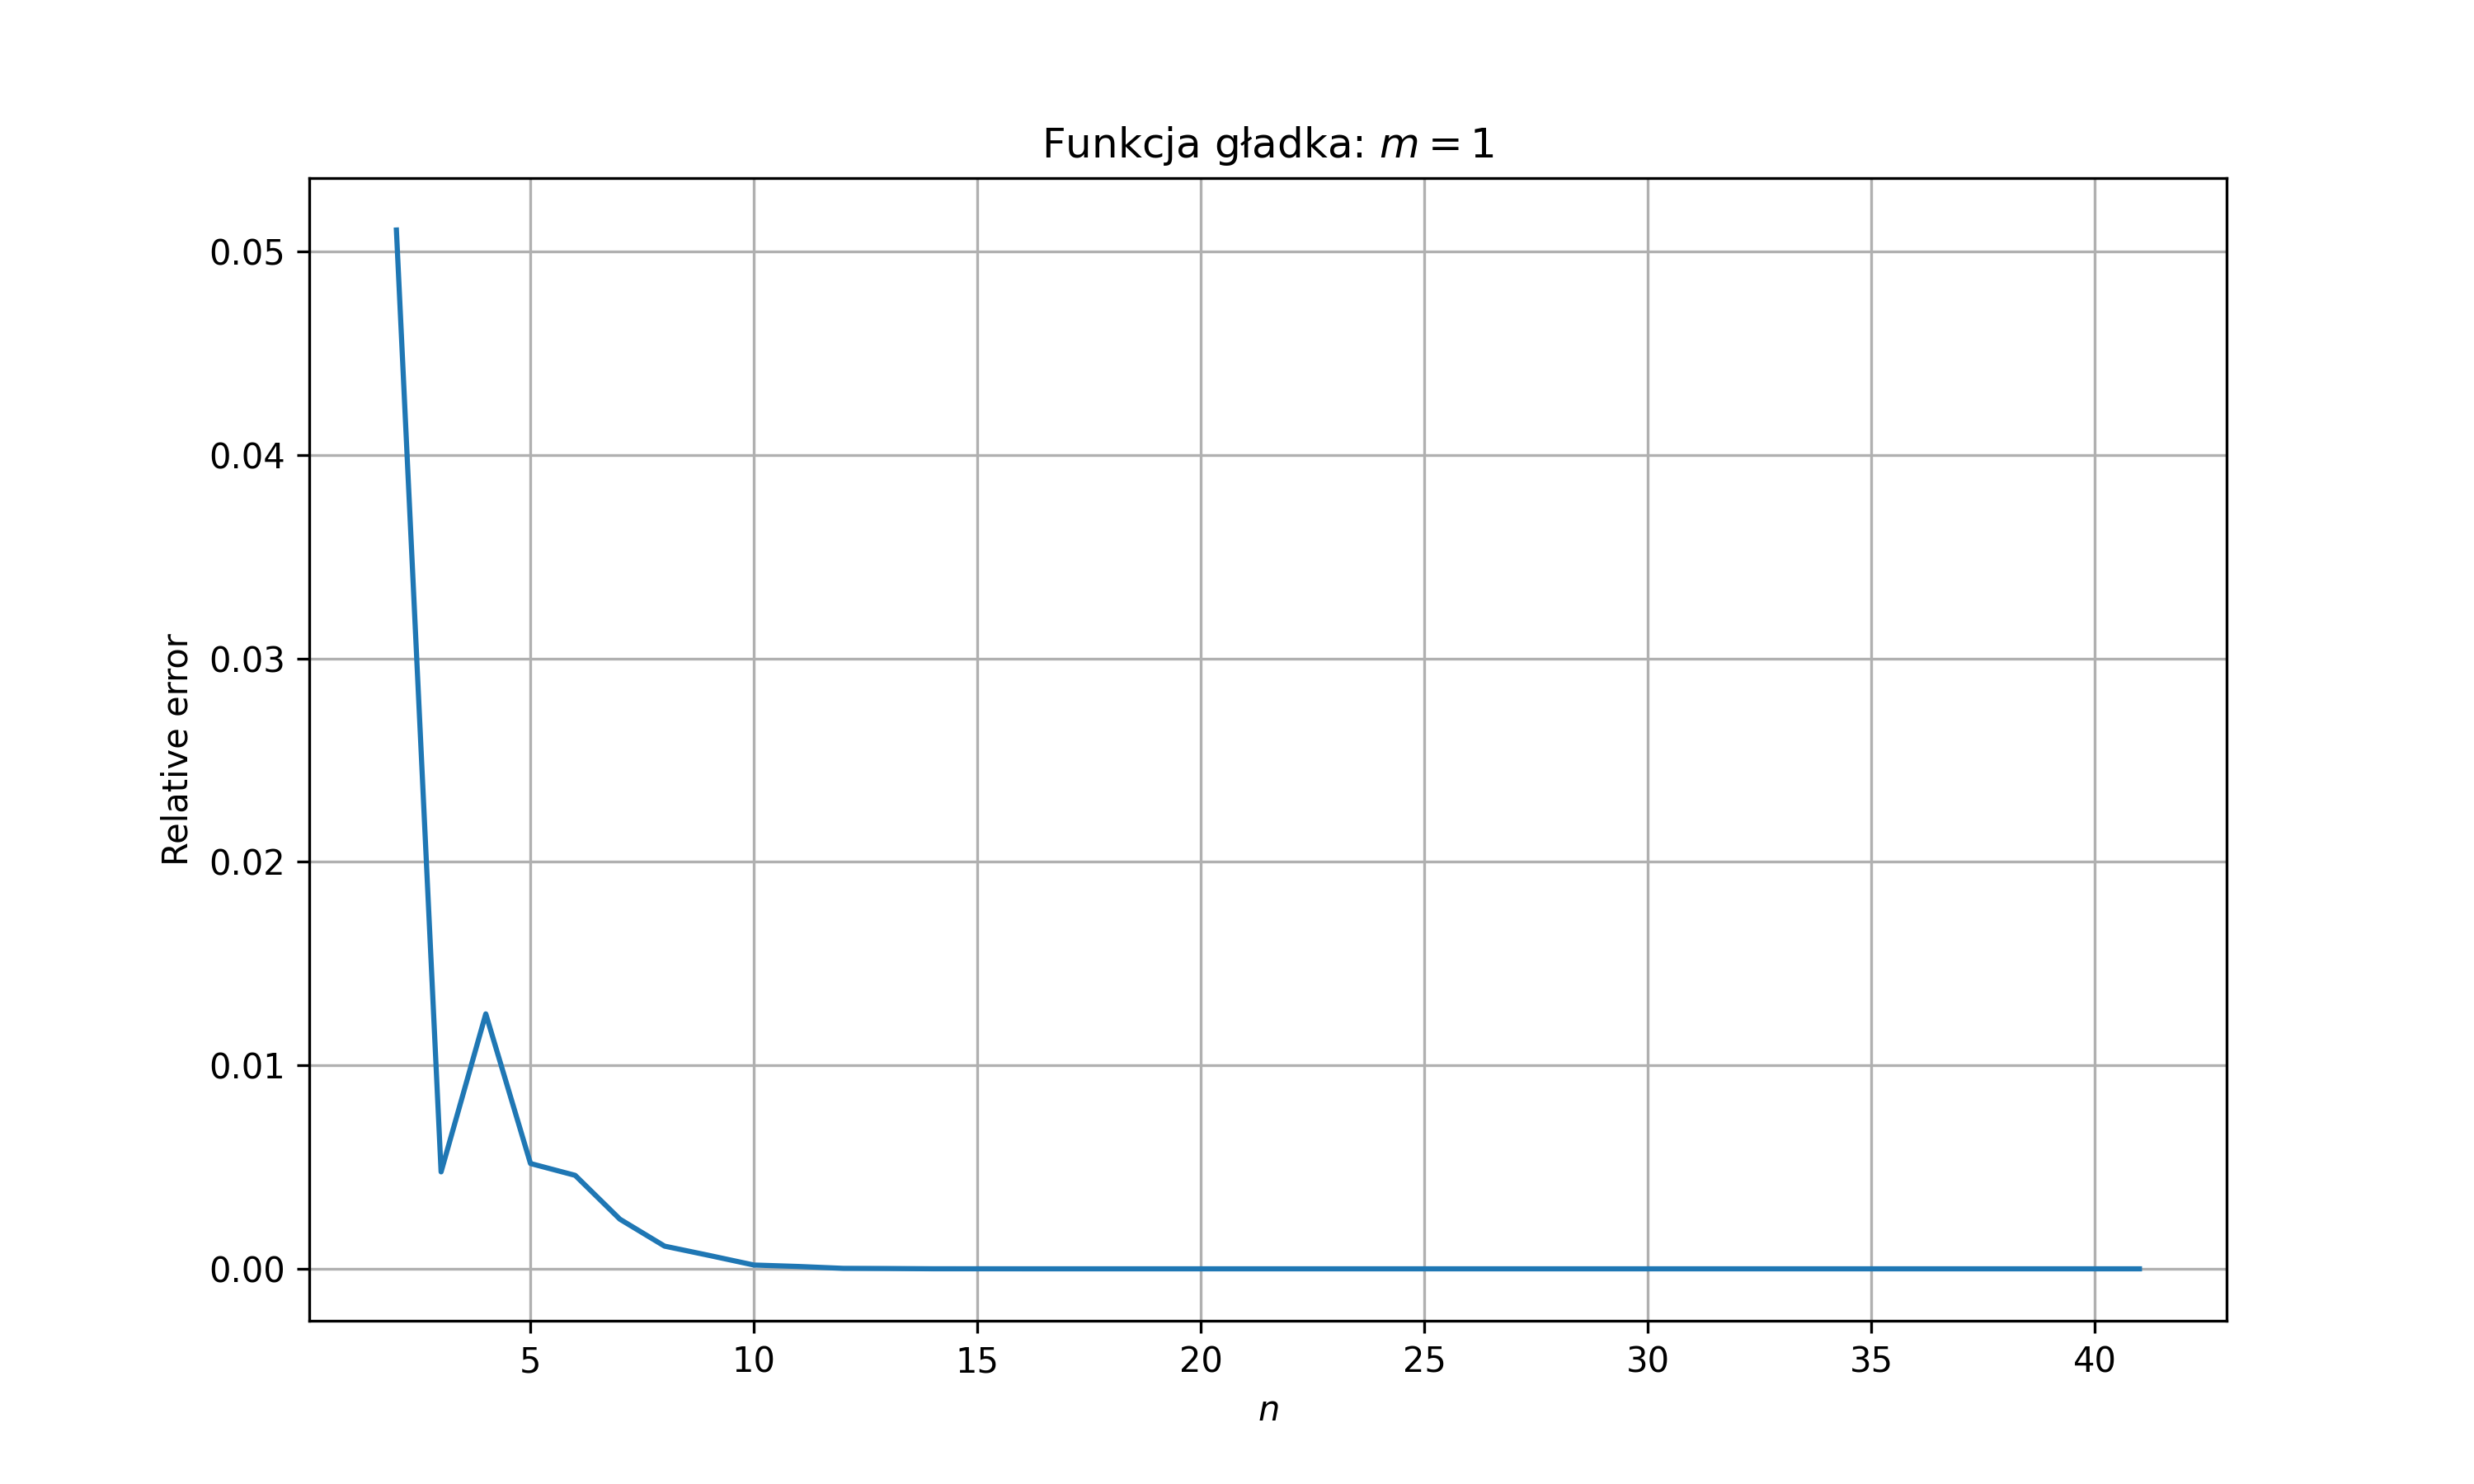
\includegraphics[width = \textwidth]{figures/task-1/smth_1.png}
\end{minipage}
\begin{minipage}{0.48\textwidth}
    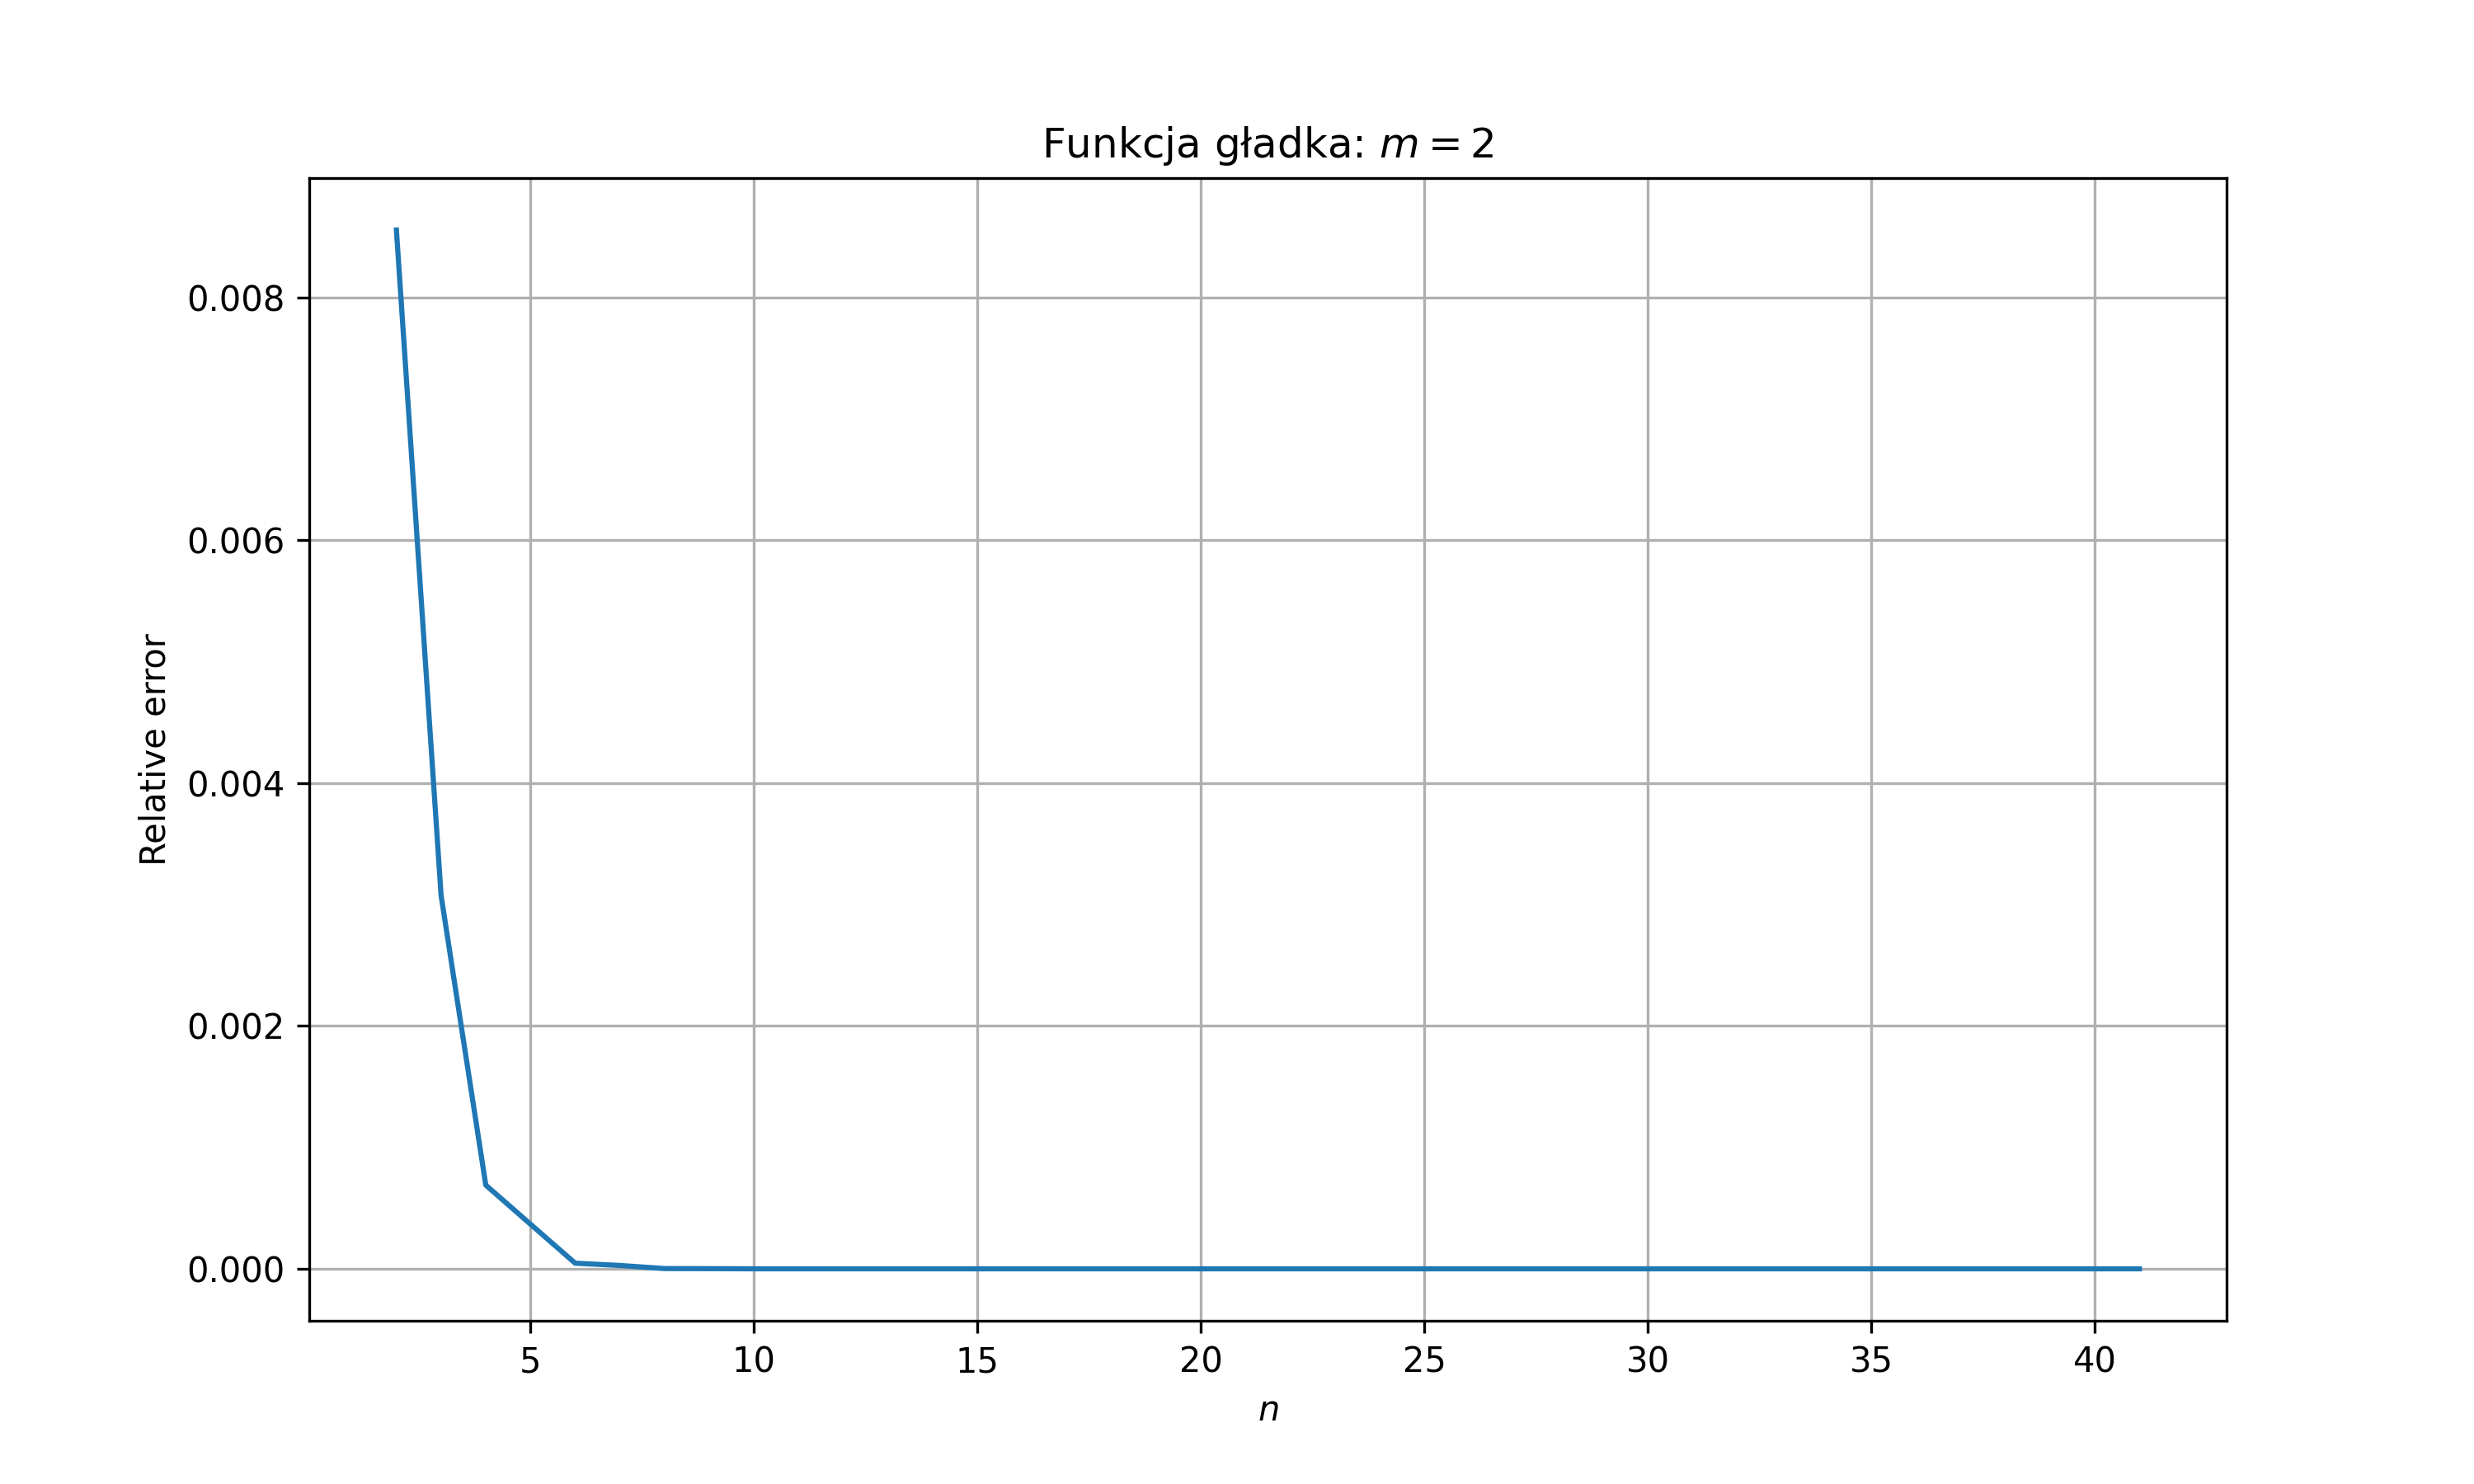
\includegraphics[width = \textwidth]{figures/task-1/smth_2.png}
\end{minipage}

\begin{minipage}{0.48\textwidth}
    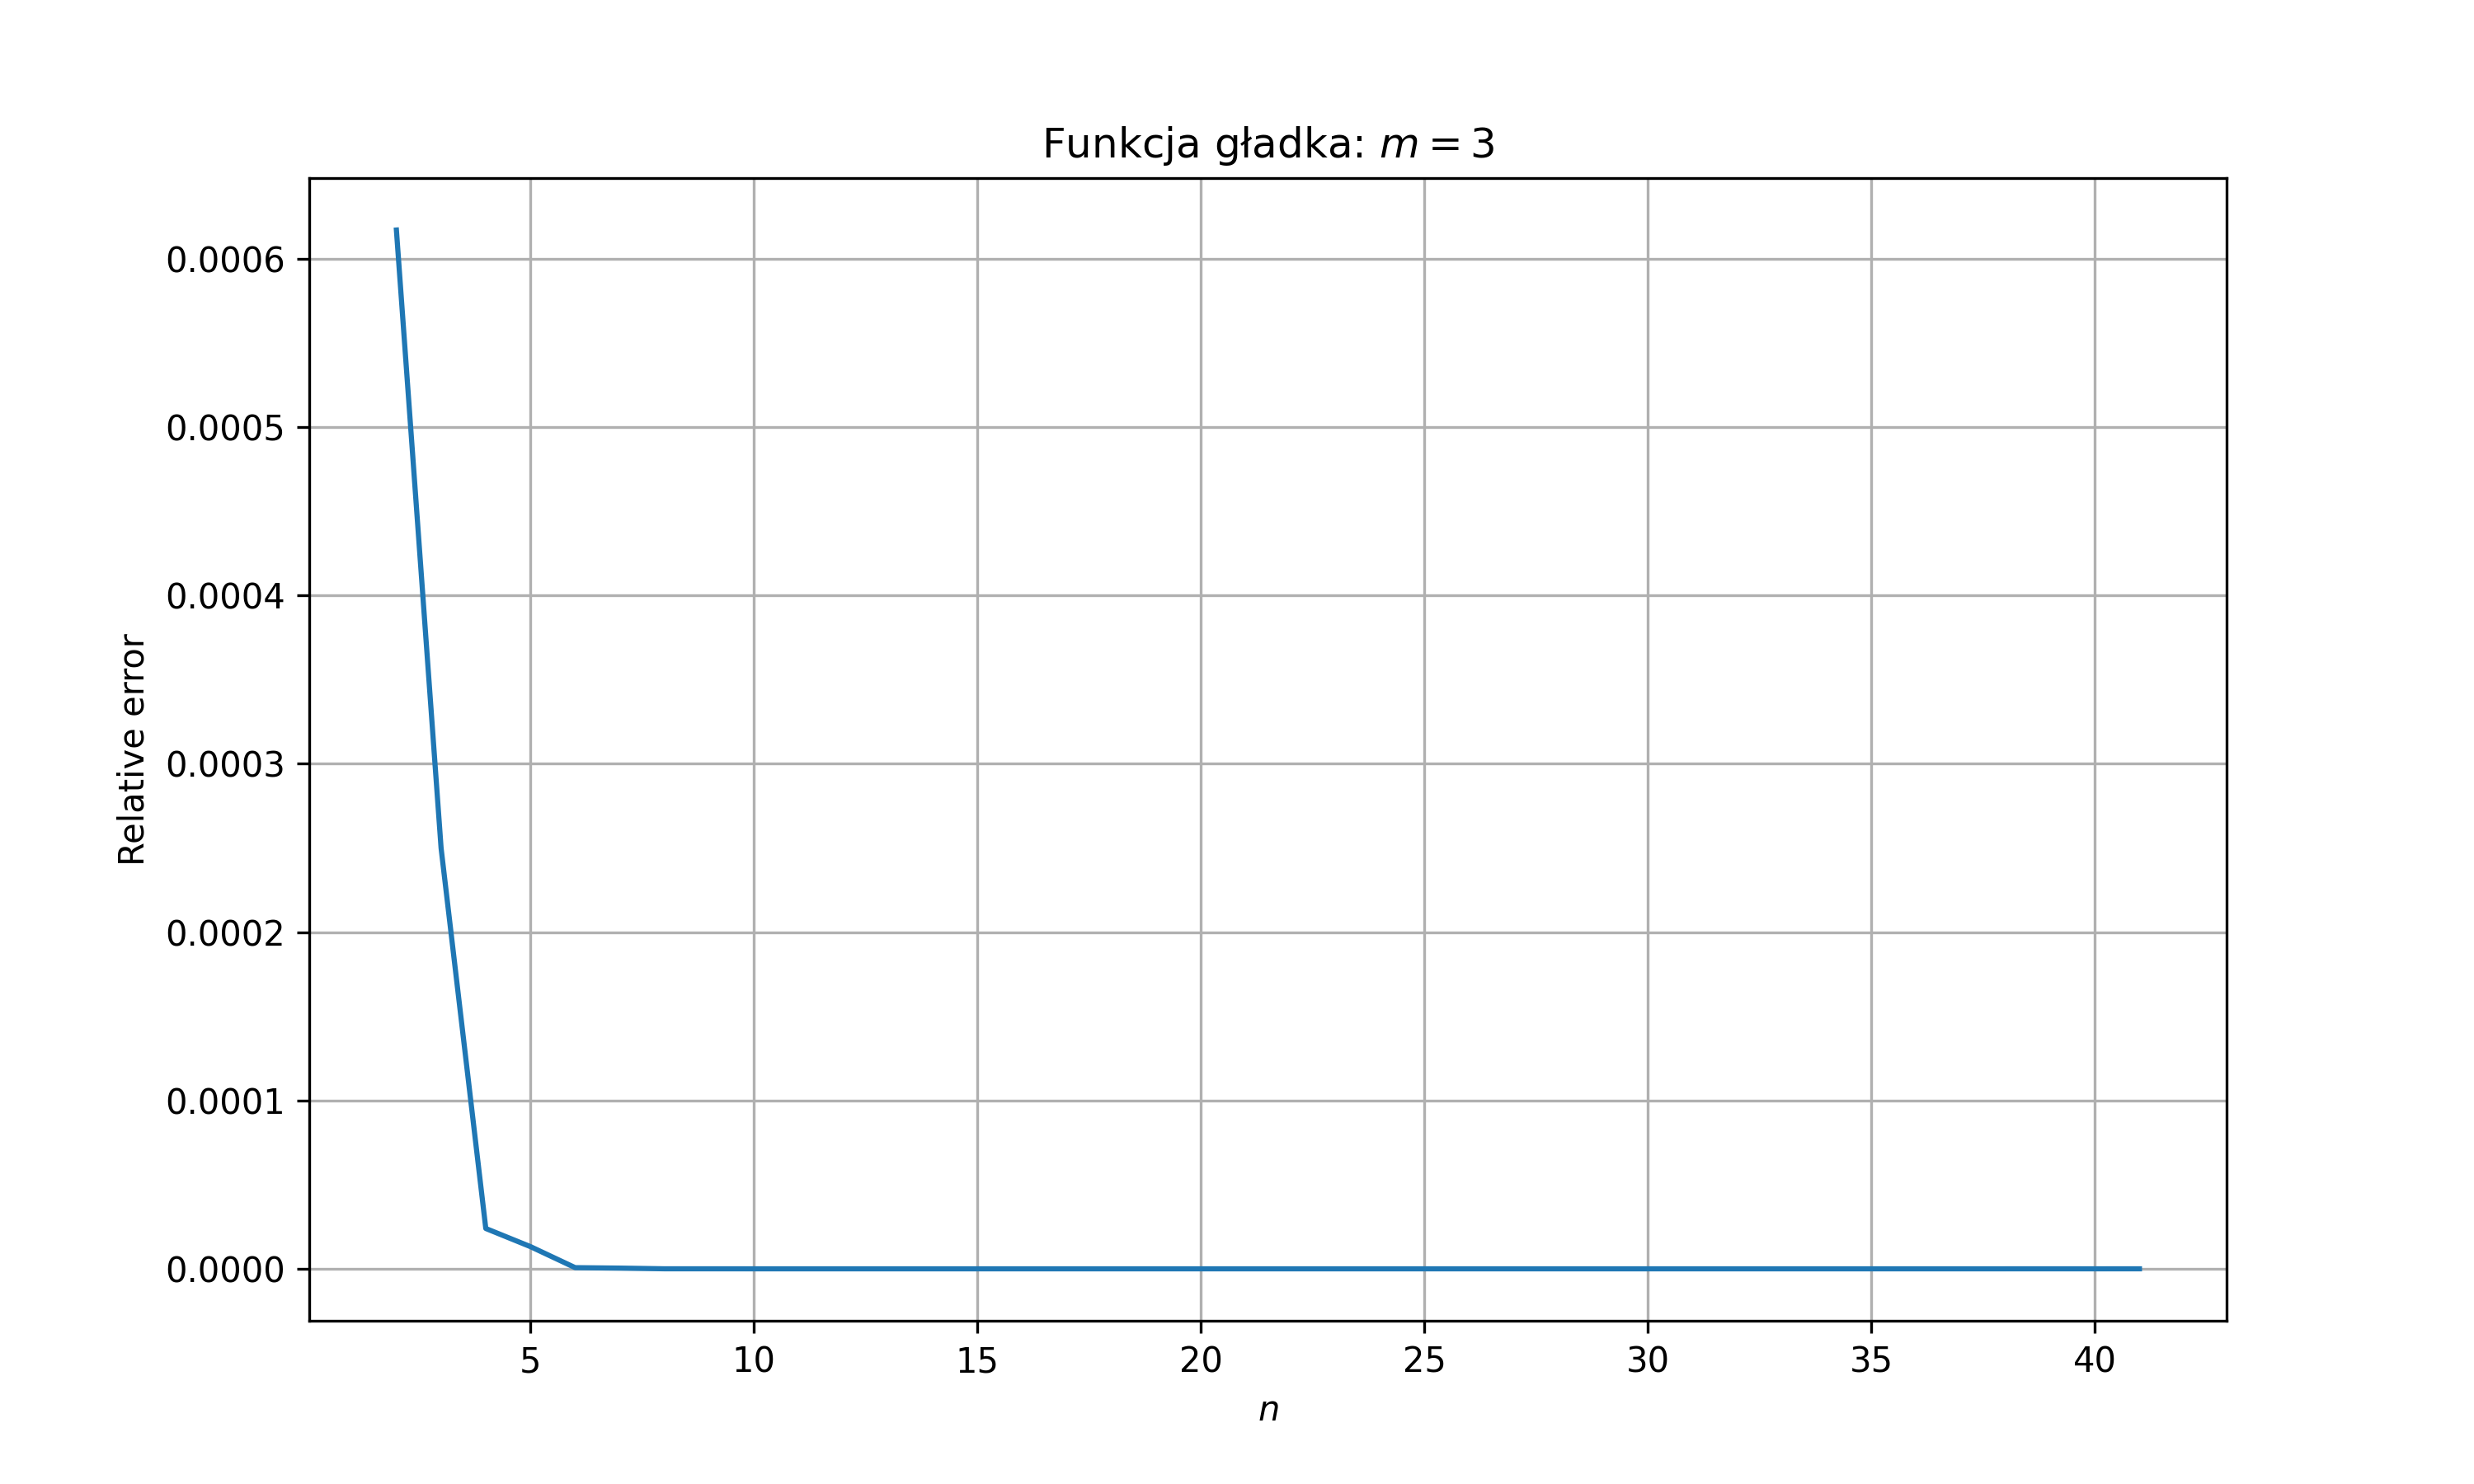
\includegraphics[width = \textwidth]{figures/task-1/smth_3.png}
\end{minipage}
\begin{minipage}{0.48\textwidth}
    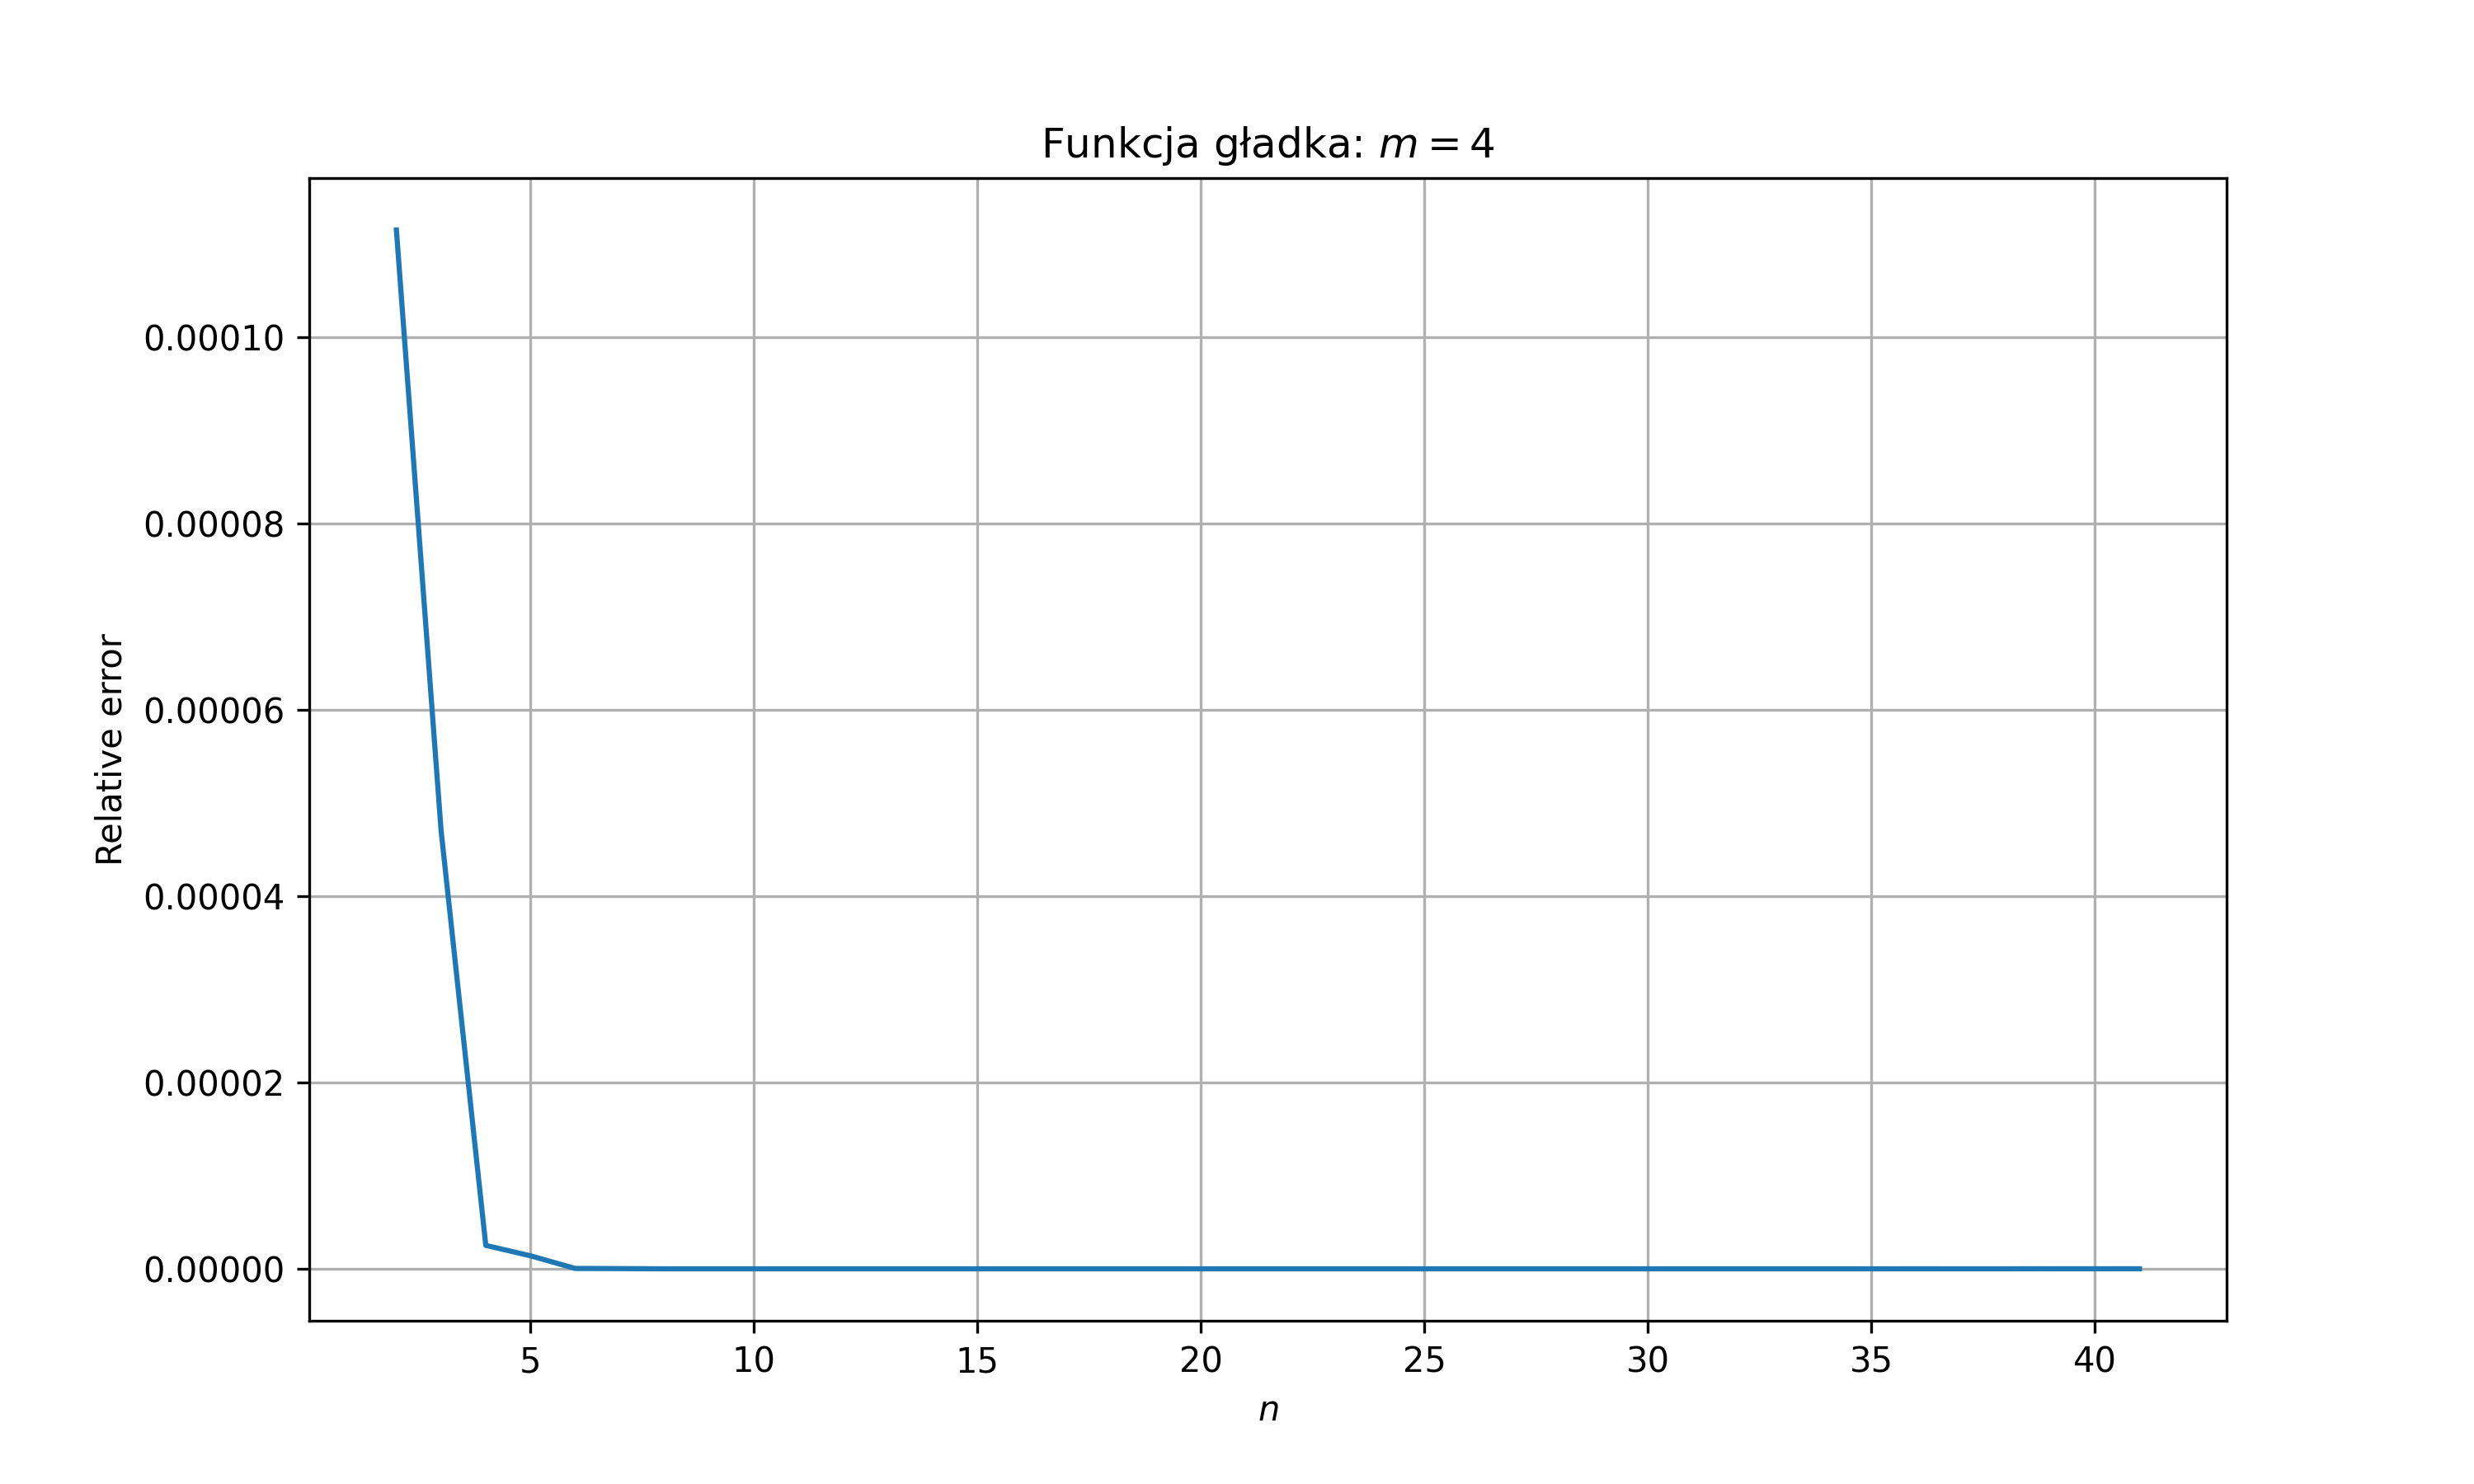
\includegraphics[width = \textwidth]{figures/task-1/smth_4.png}
\end{minipage}
Absolute error

\paragraph{Nonuniformly continuous function}
\indent

\begin{minipage}{0.48\textwidth}
    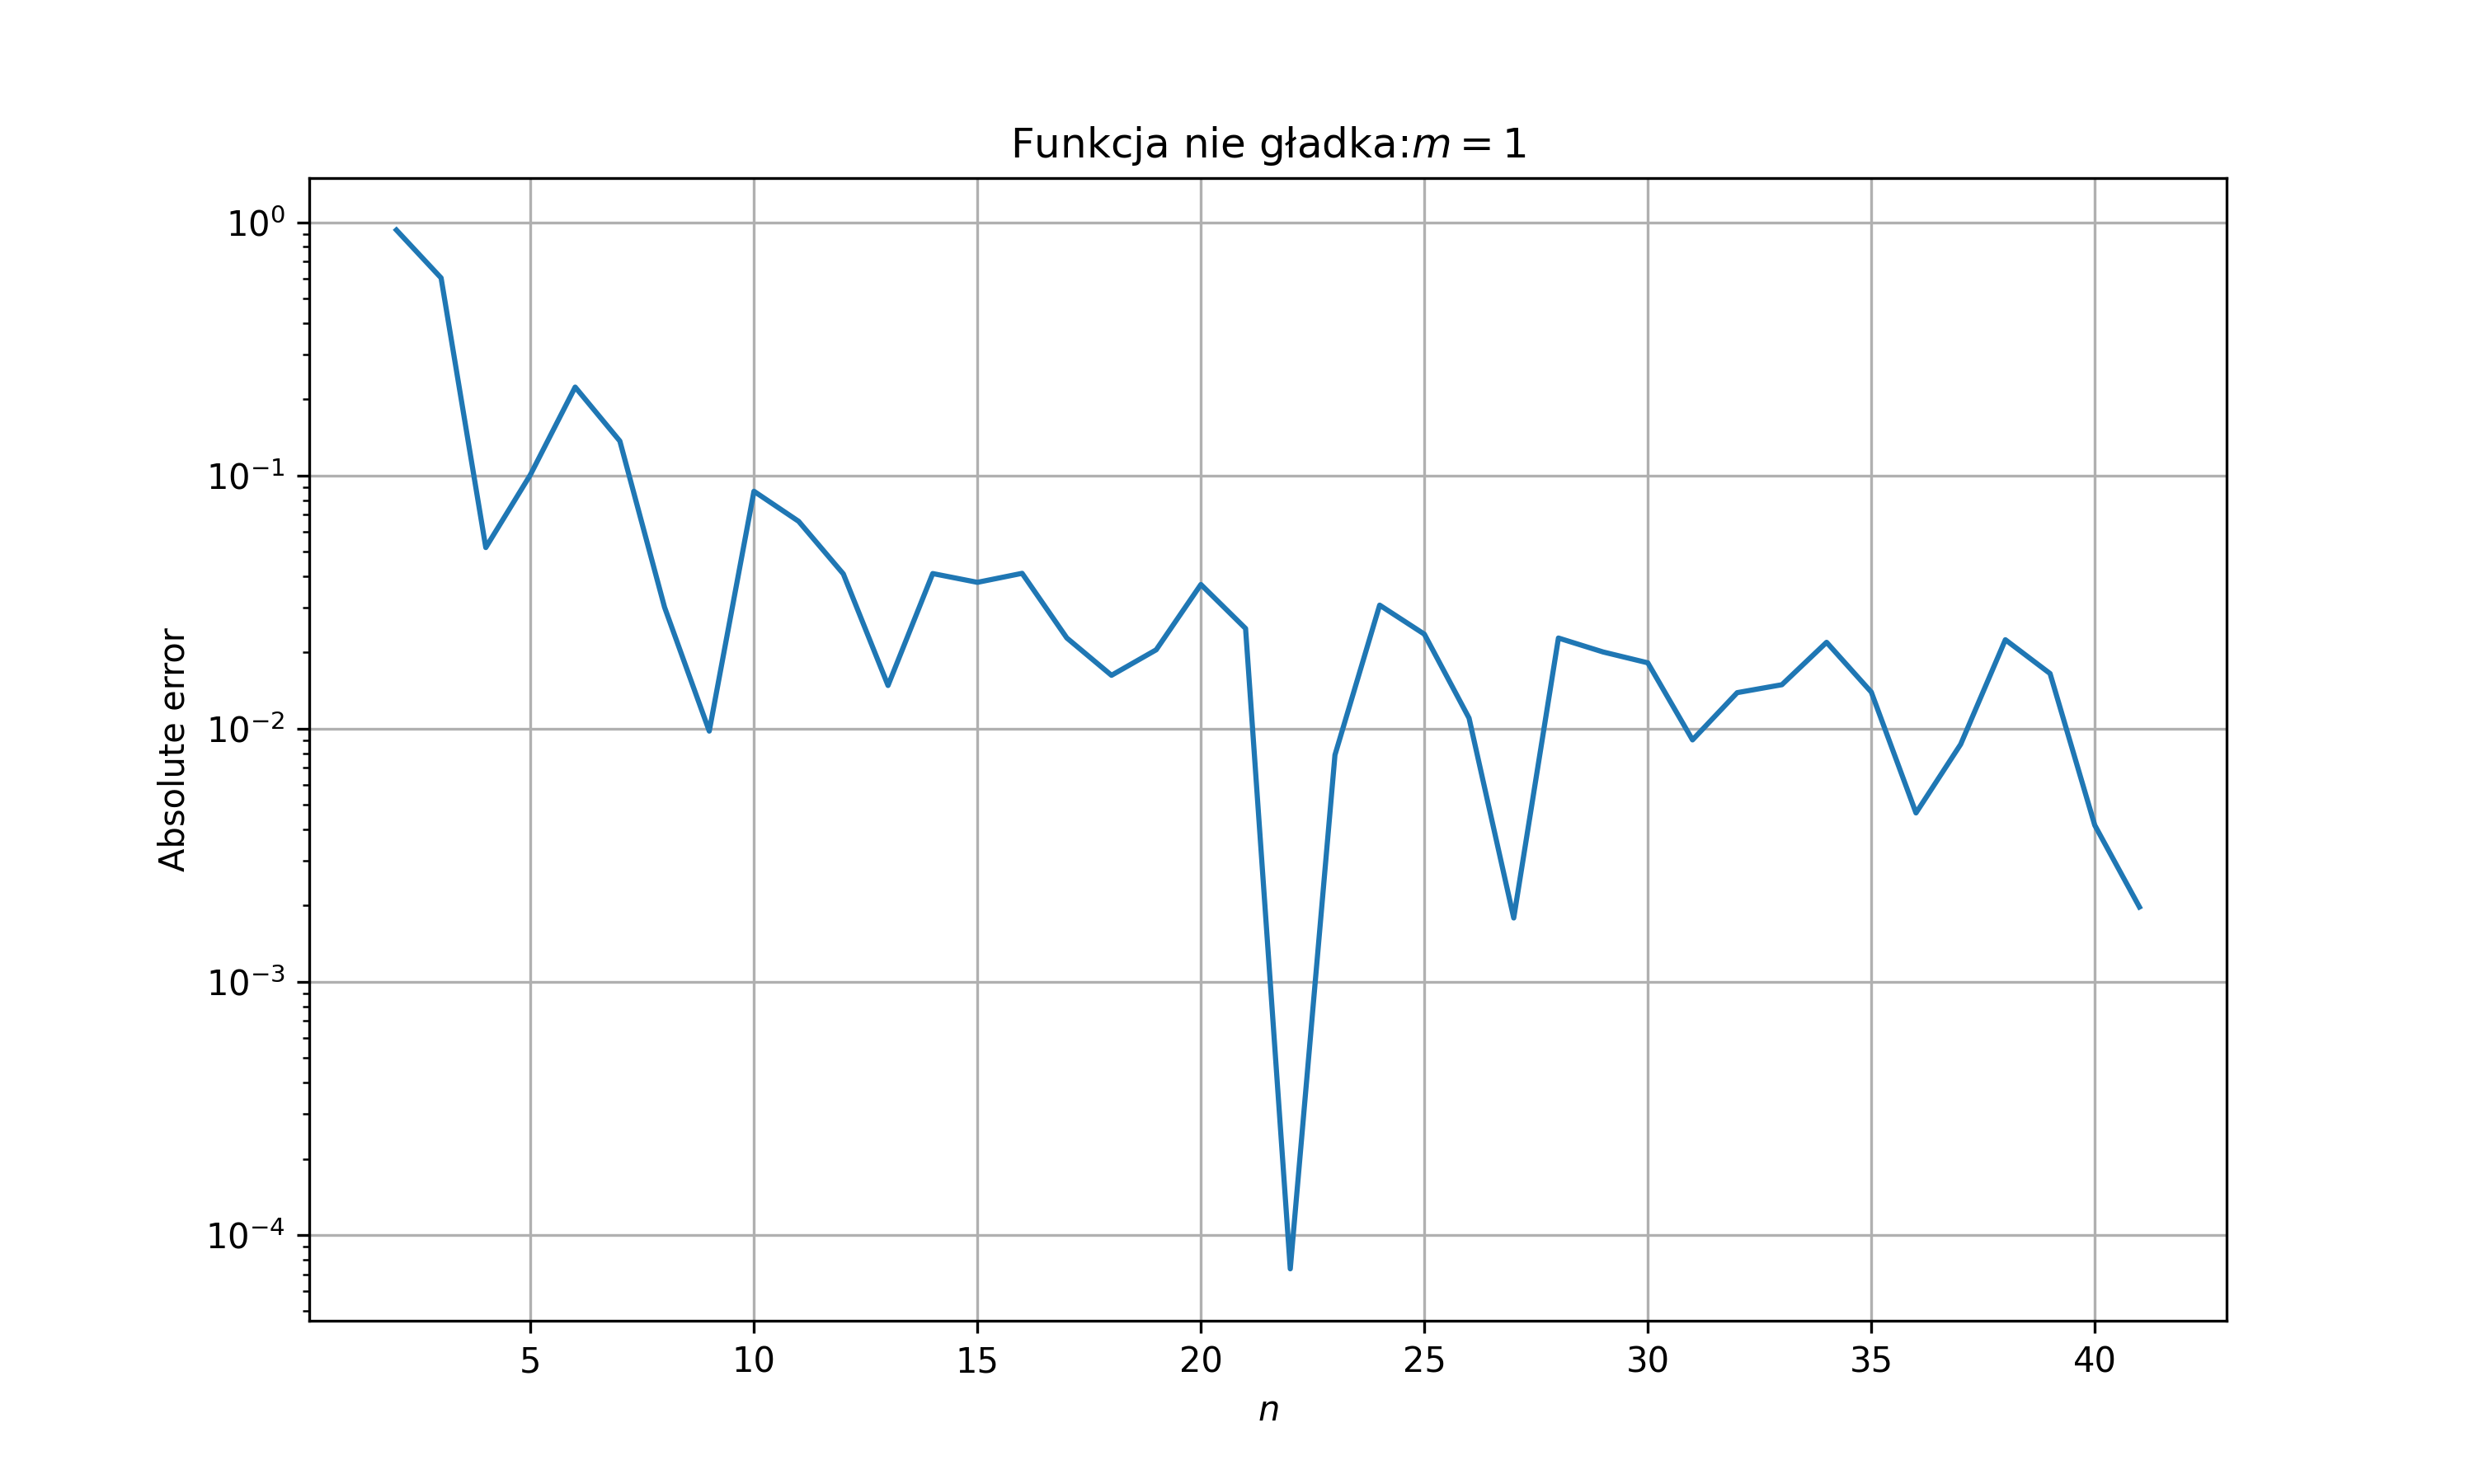
\includegraphics[width = \textwidth]{figures/task-1/abs_nsmth_1.png}
\end{minipage}
\begin{minipage}{0.48\textwidth}
    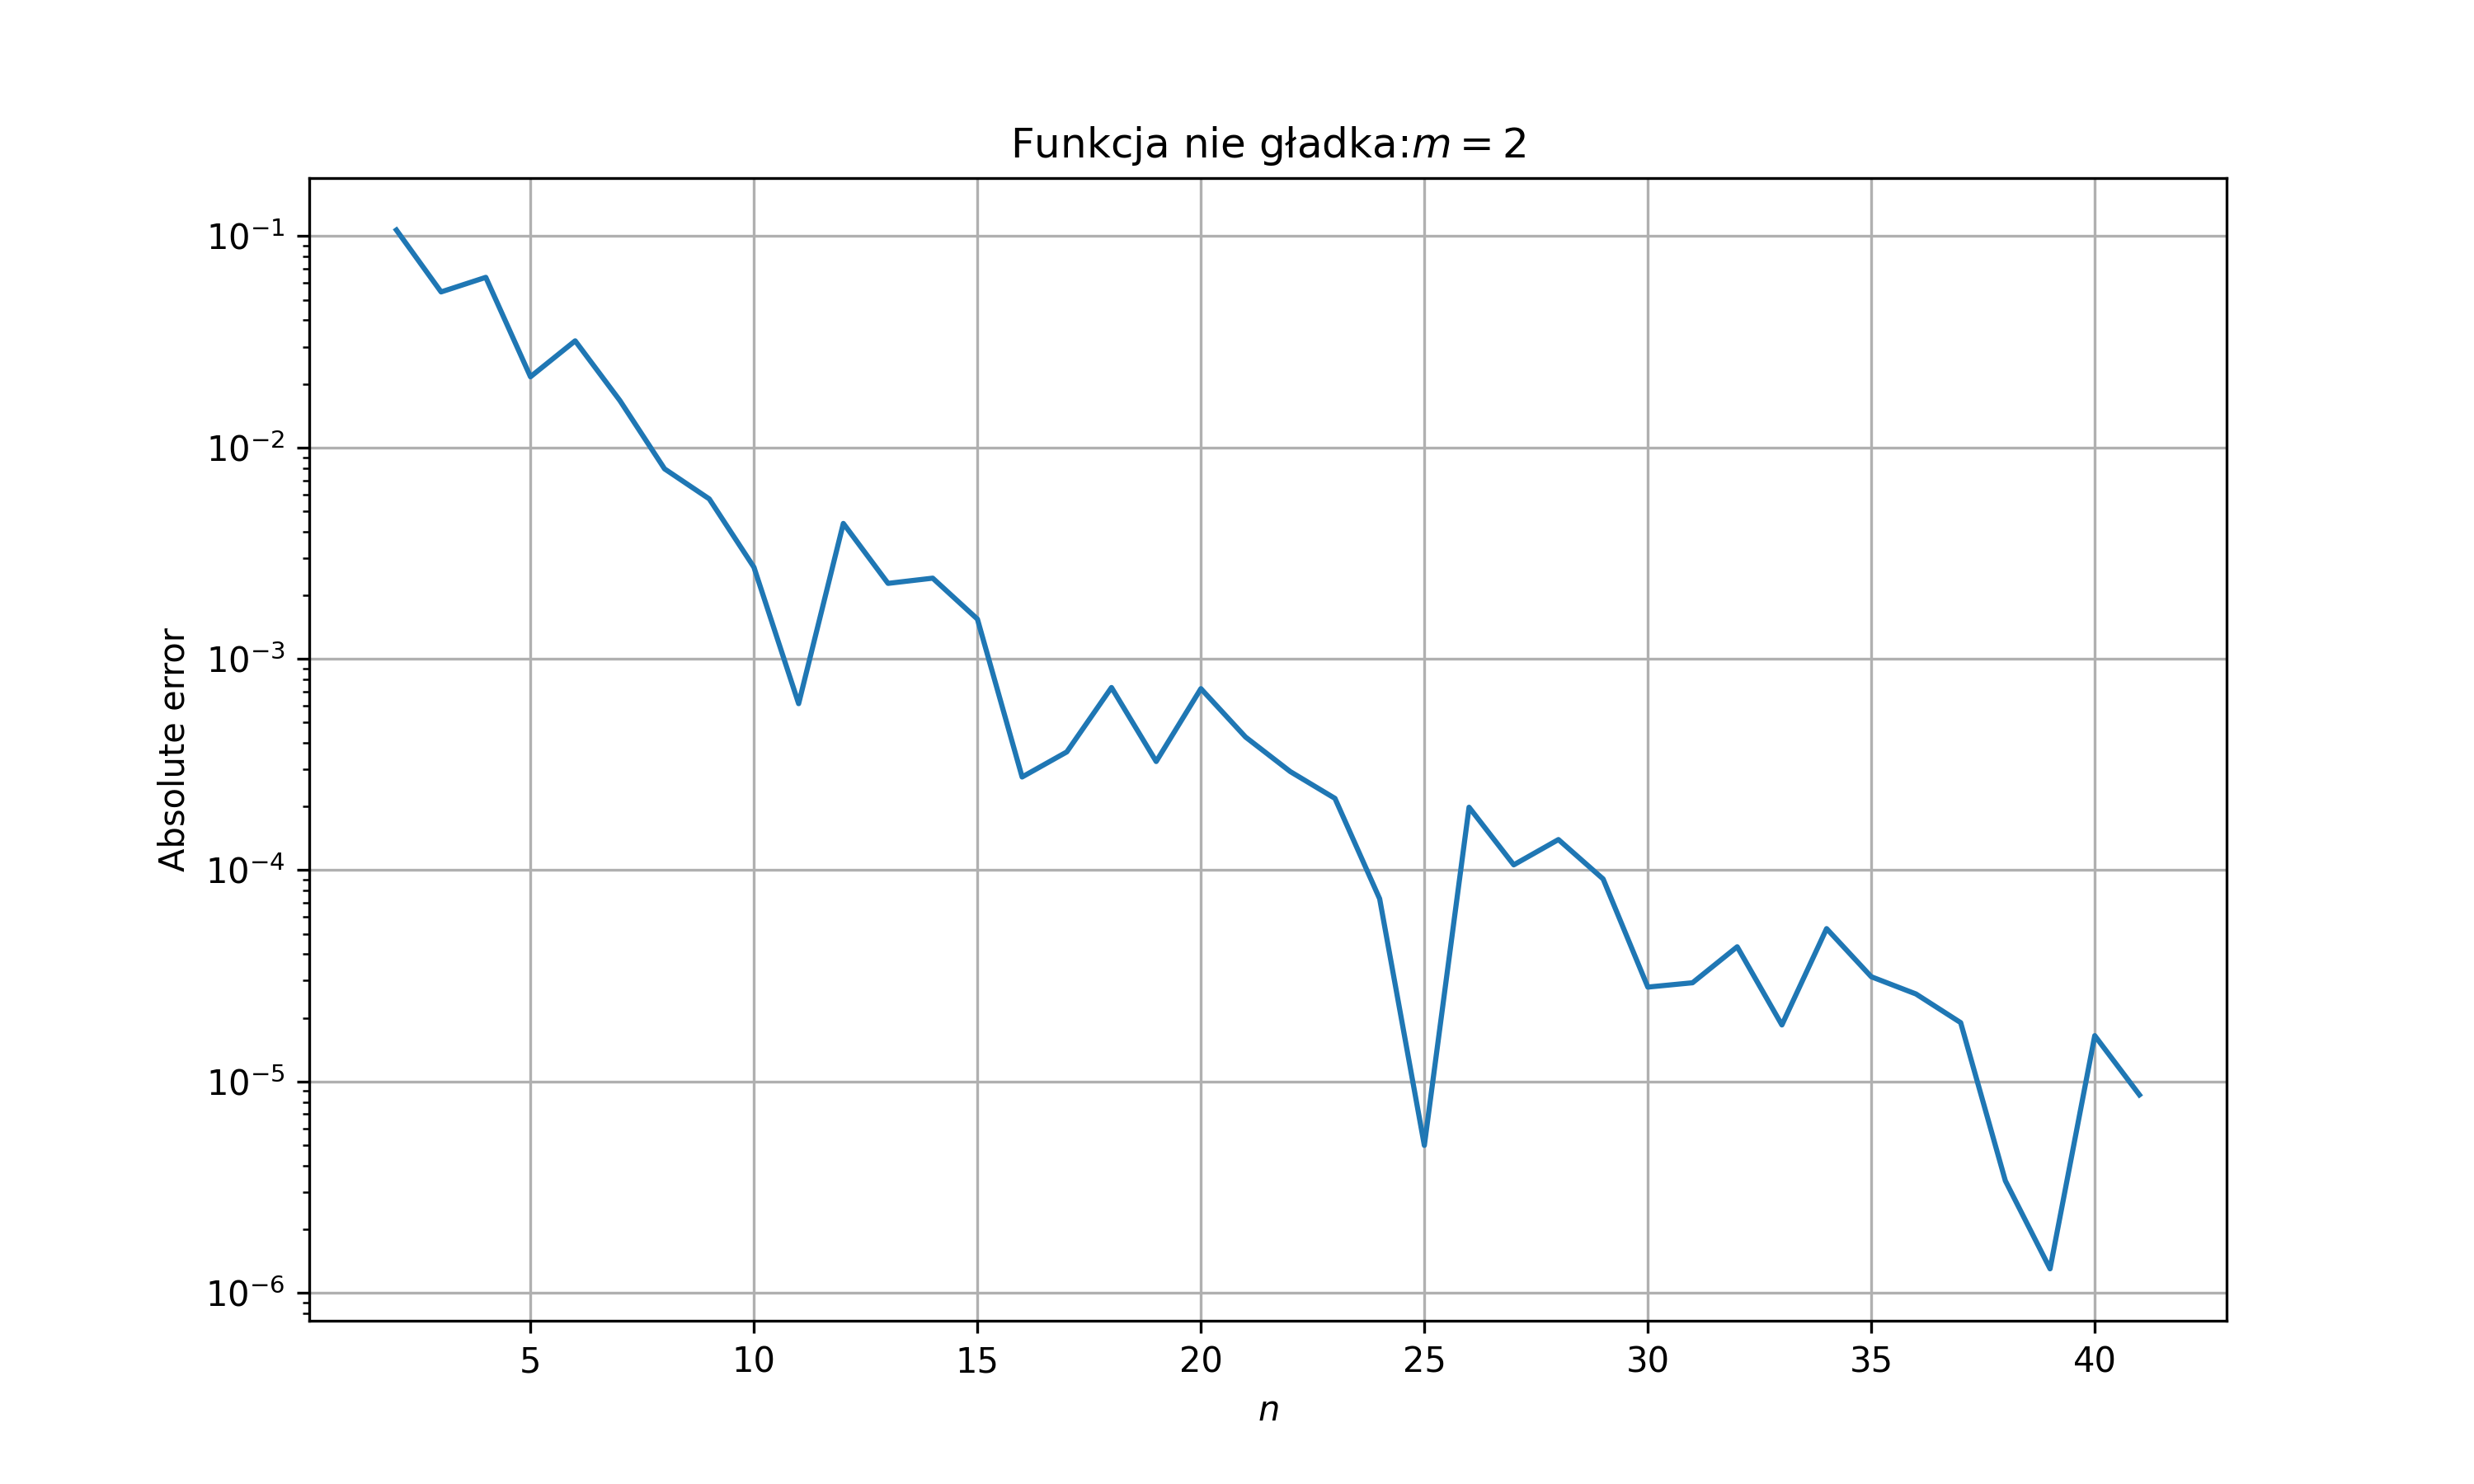
\includegraphics[width = \textwidth]{figures/task-1/abs_nsmth_2.png}
\end{minipage}

\begin{minipage}{0.48\textwidth}
    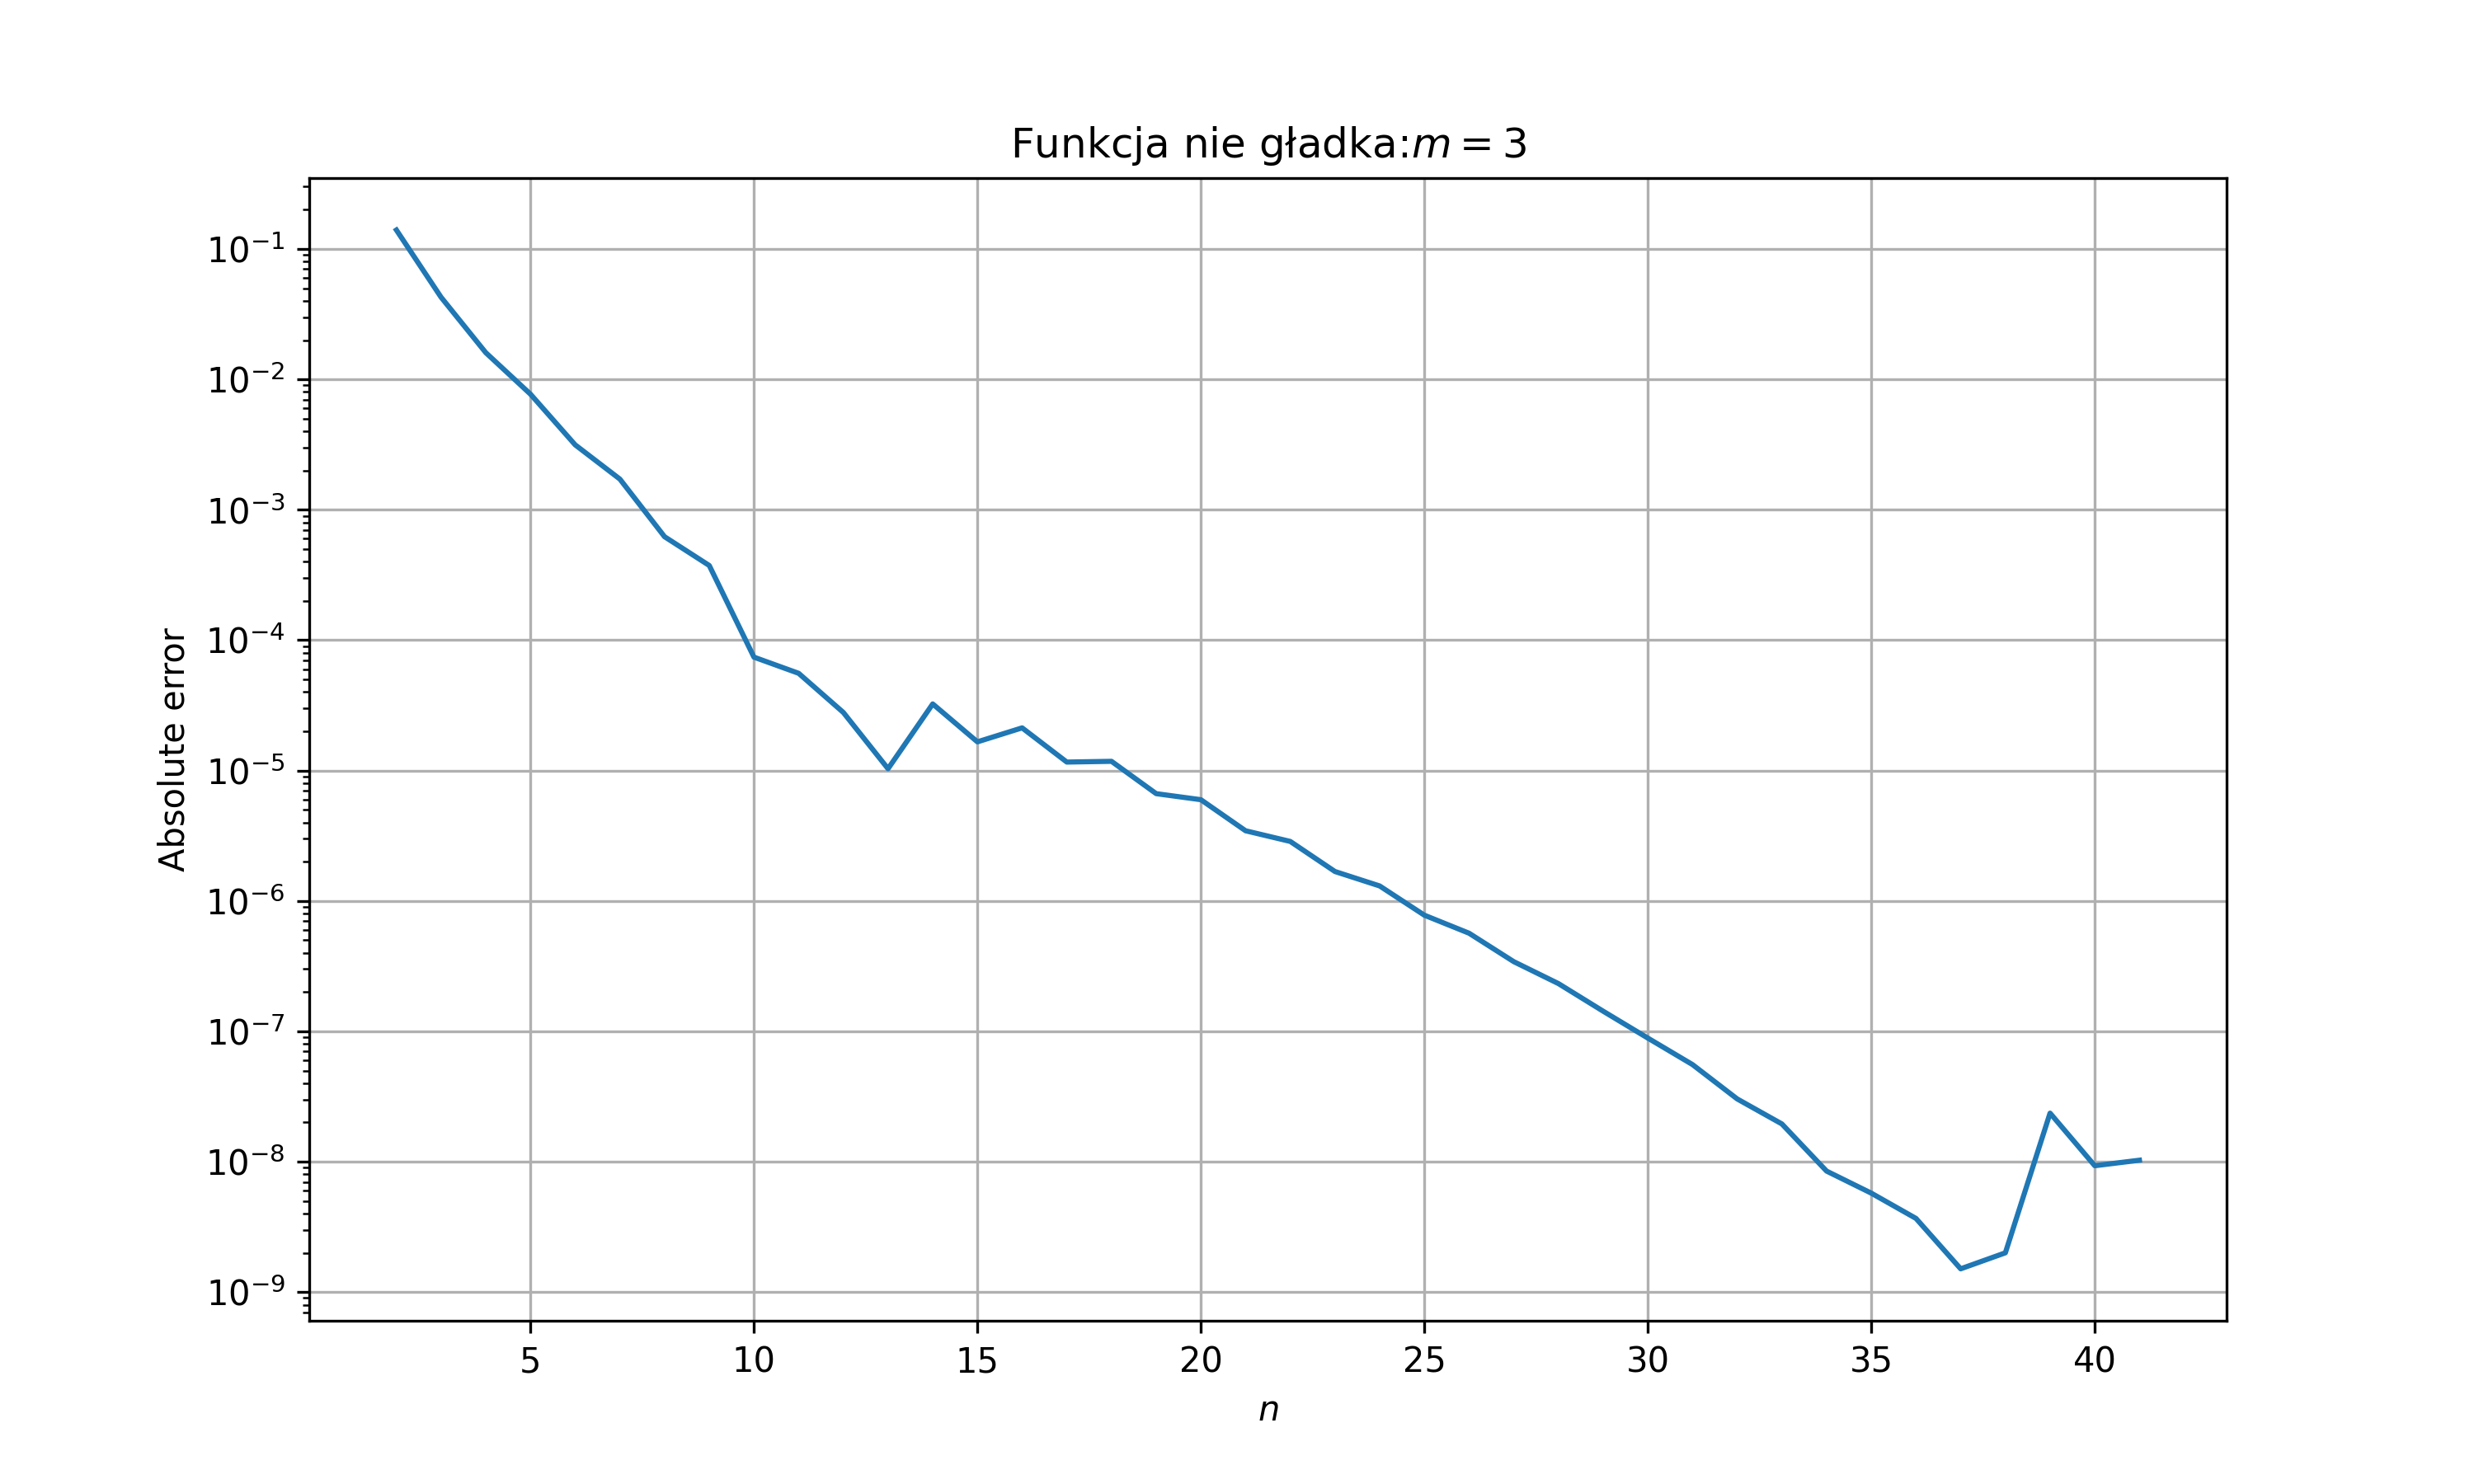
\includegraphics[width = \textwidth]{figures/task-1/abs_nsmth_3.png}
\end{minipage}
\begin{minipage}{0.48\textwidth}
    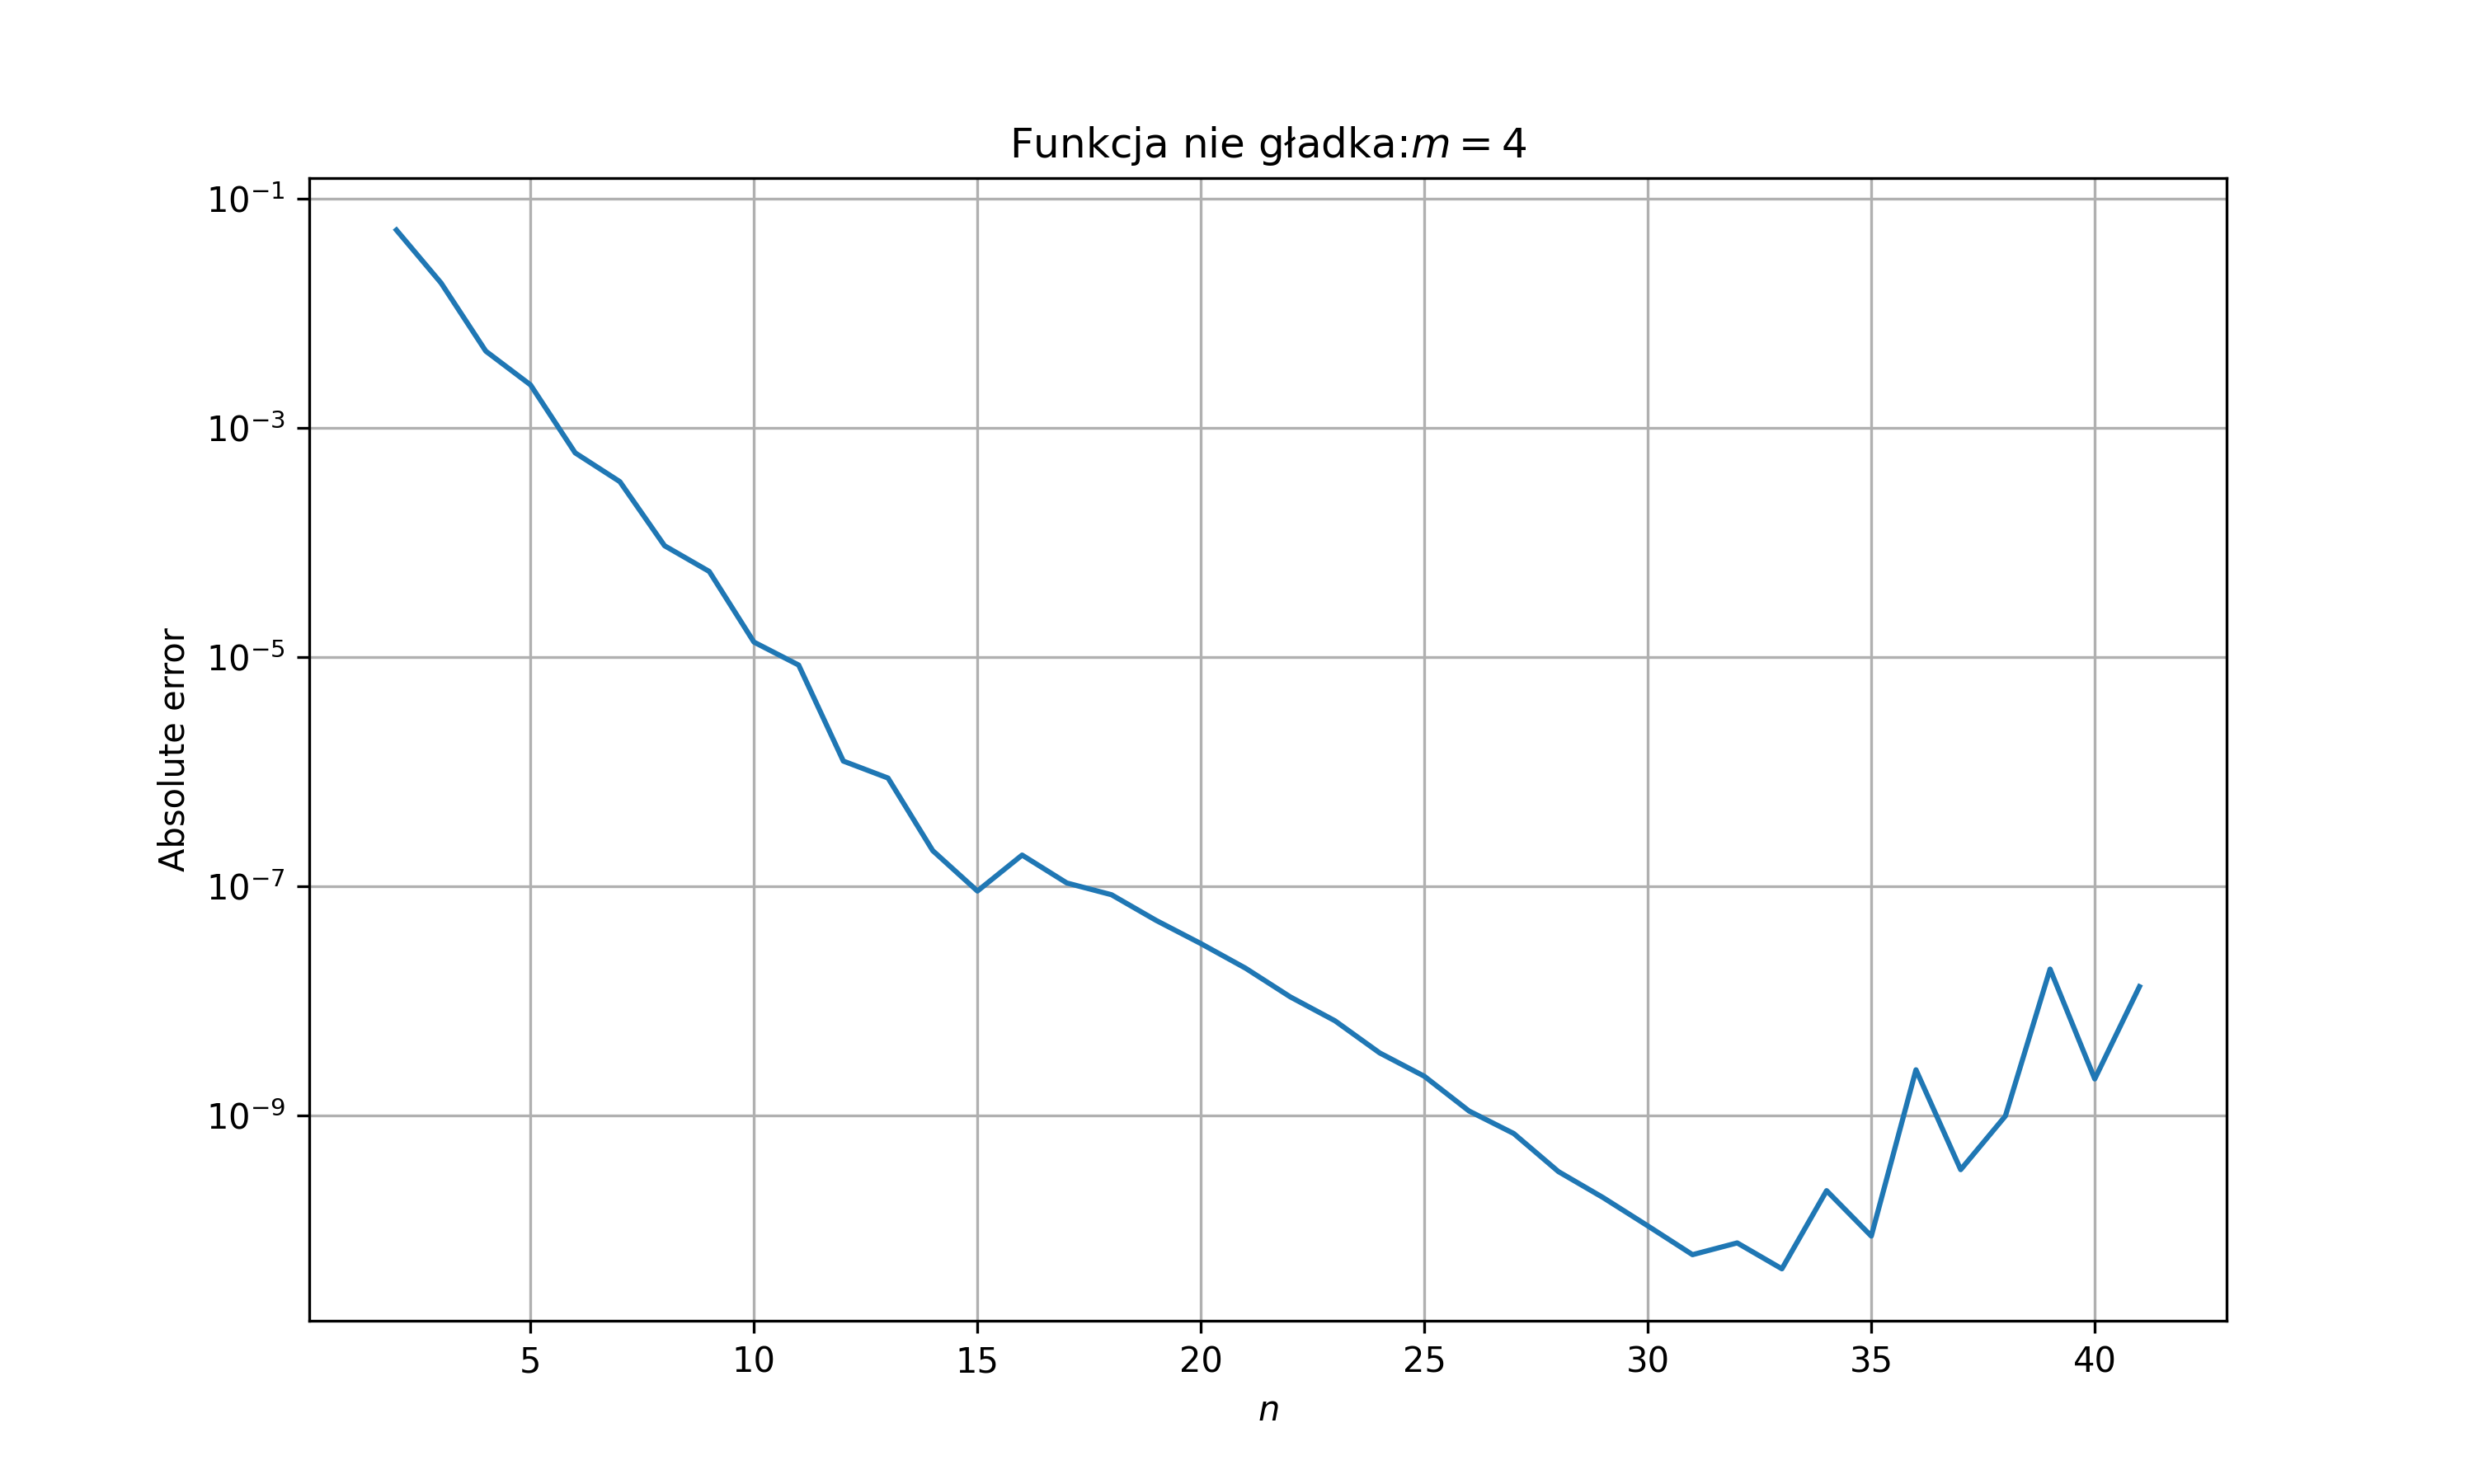
\includegraphics[width = \textwidth]{figures/task-1/abs_nsmth_4.png}
\end{minipage}
Relative error

\begin{minipage}{0.48\textwidth}
    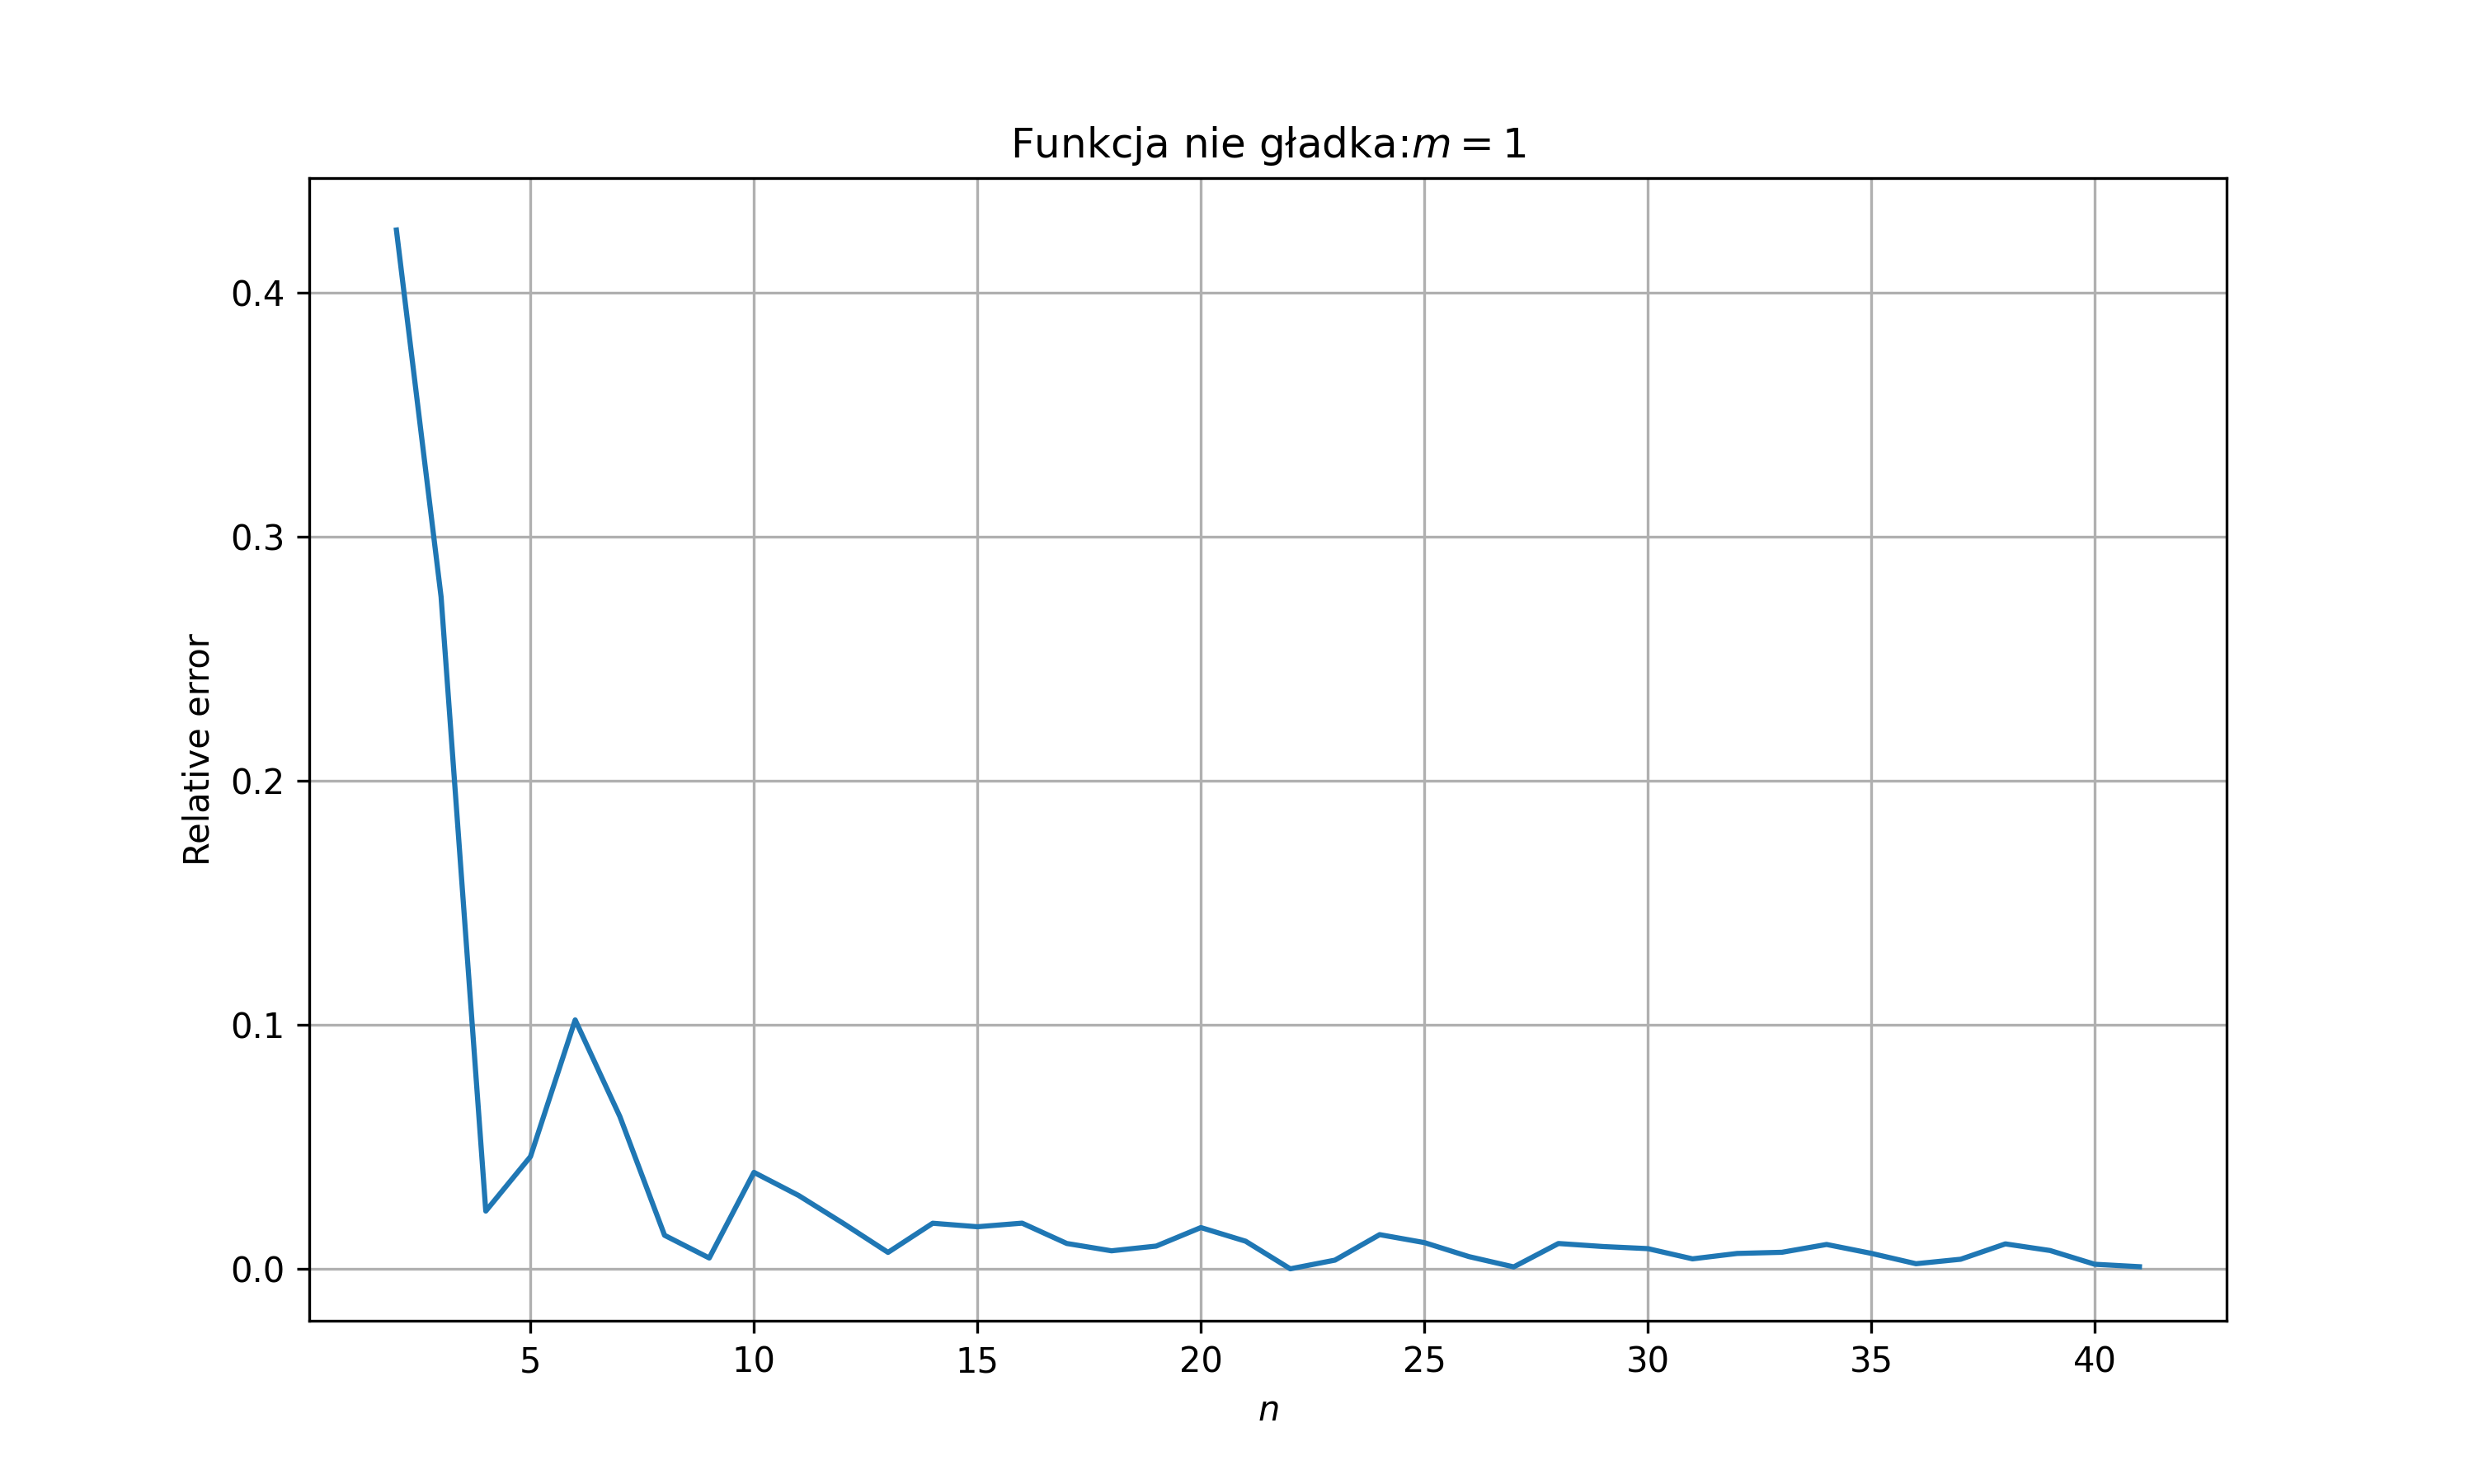
\includegraphics[width = \textwidth]{figures/task-1/nsmth_1.png}
\end{minipage}
\begin{minipage}{0.48\textwidth}
    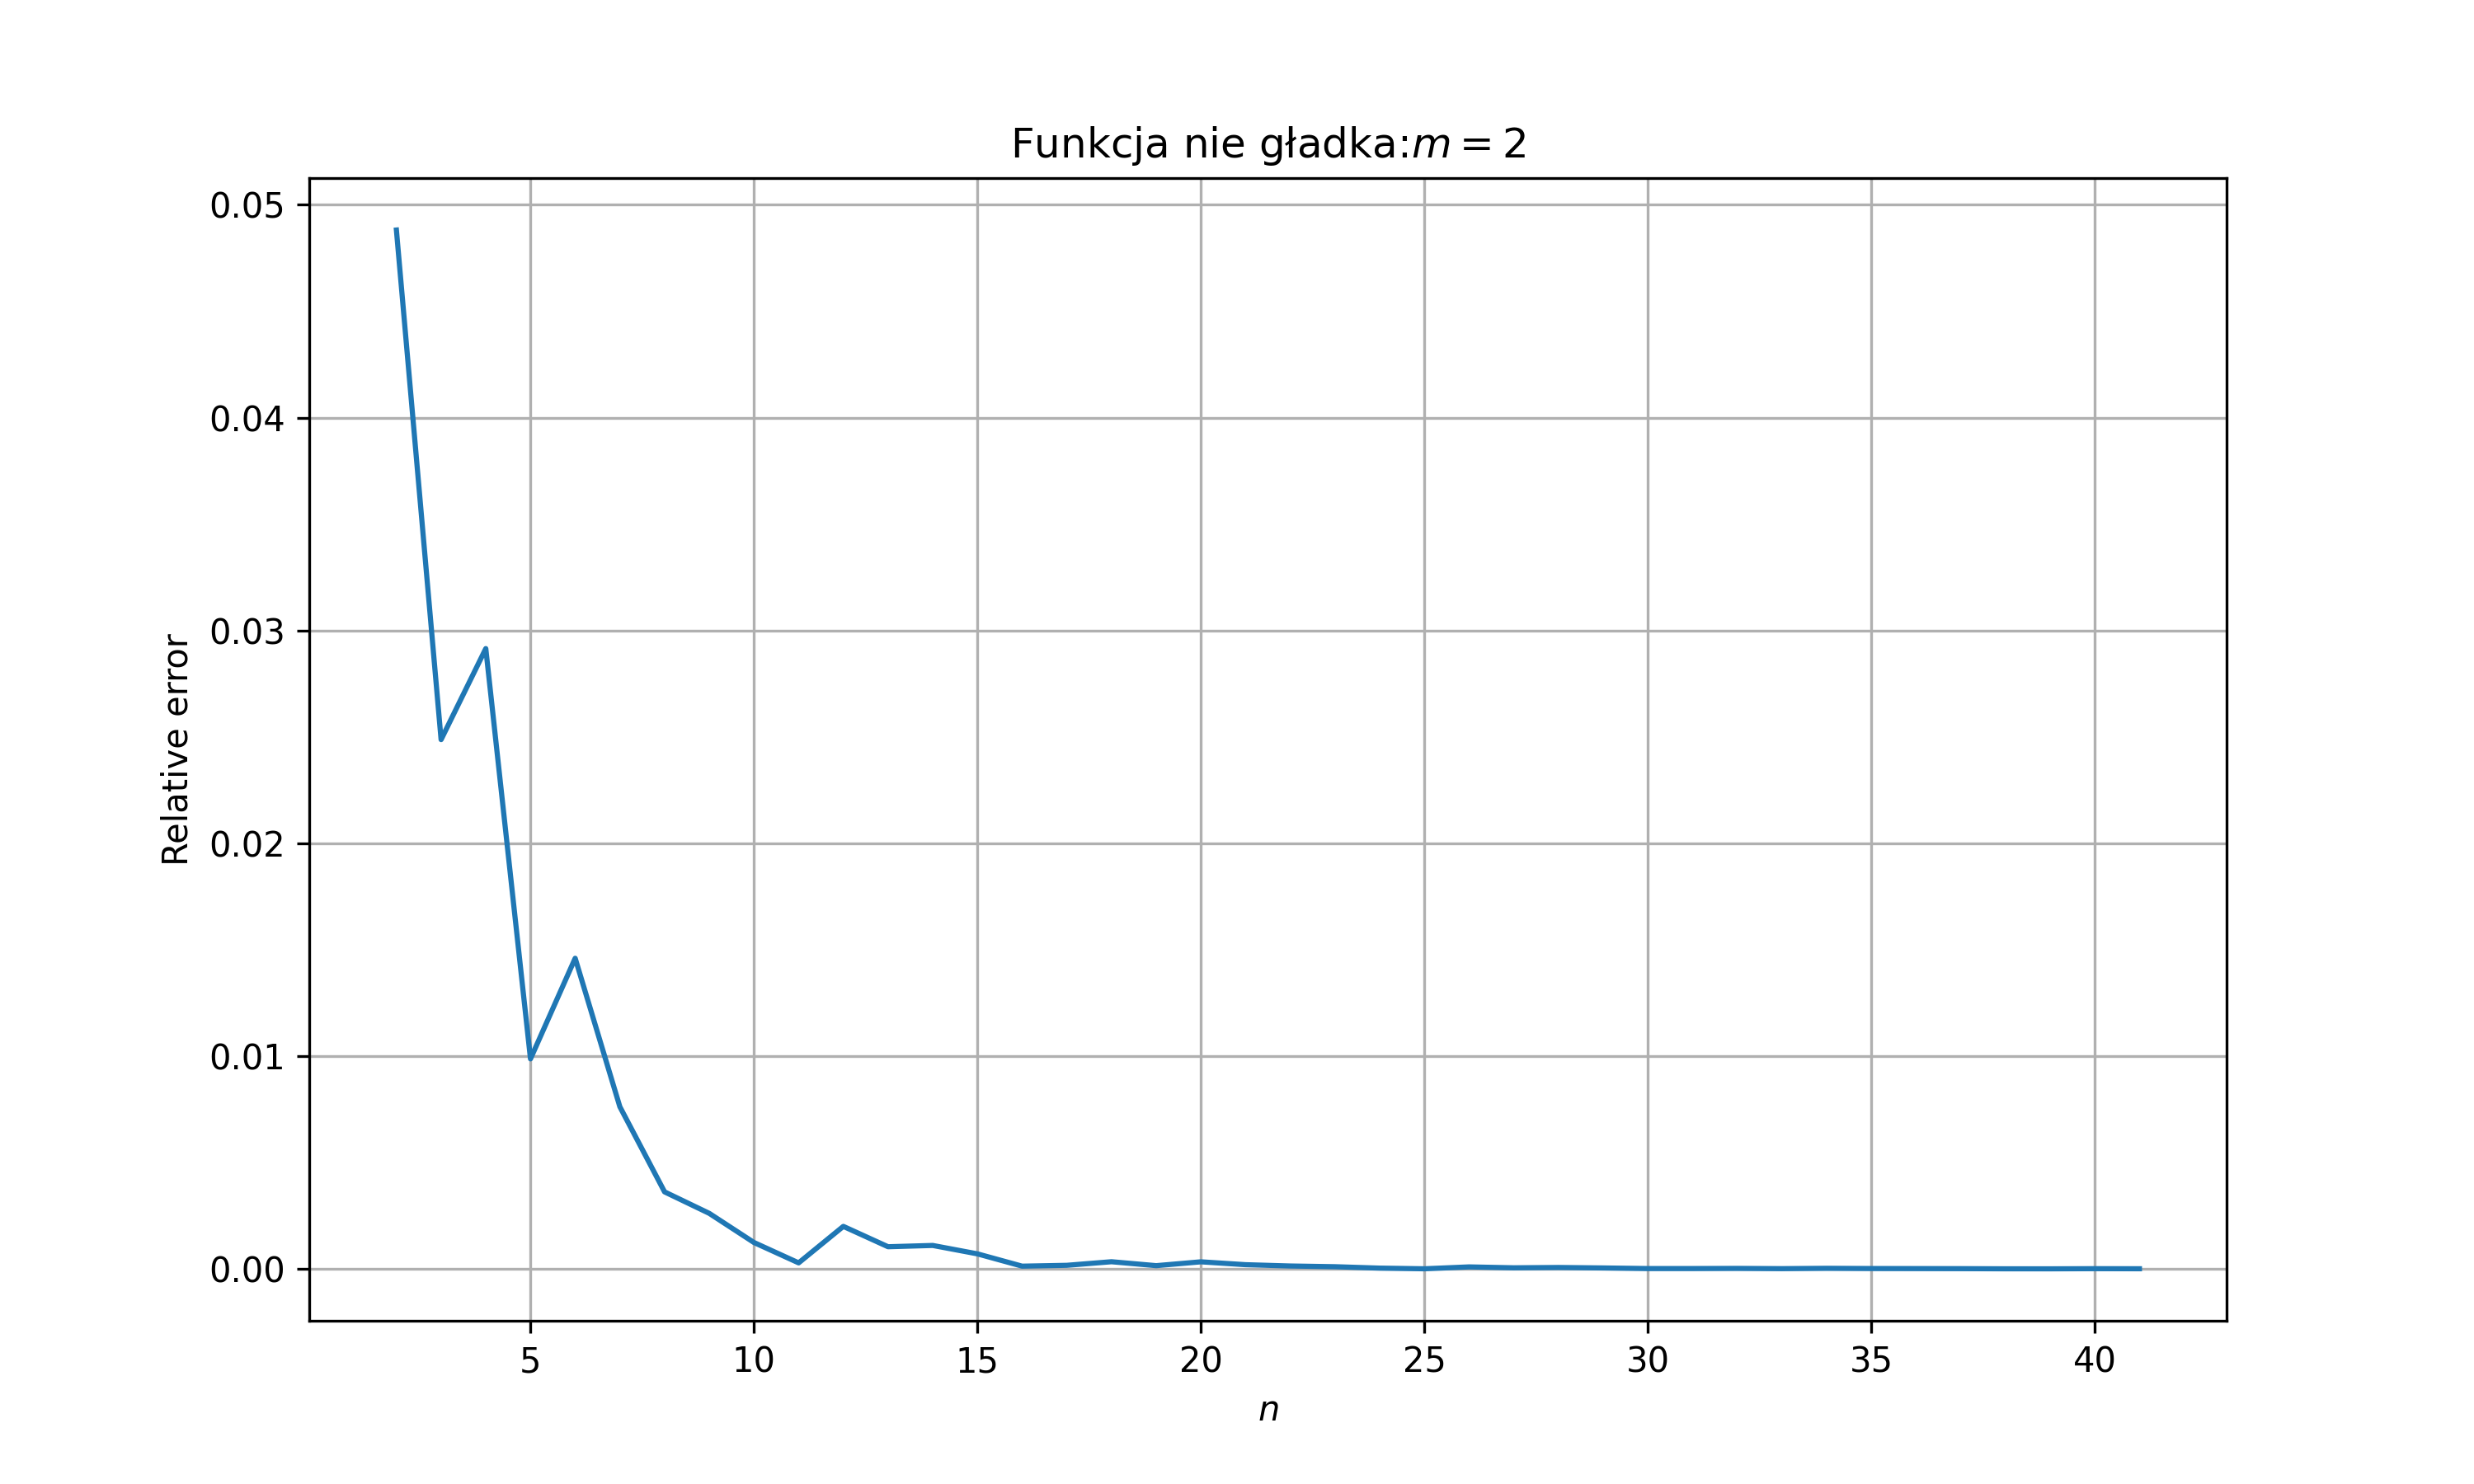
\includegraphics[width = \textwidth]{figures/task-1/nsmth_2.png}
\end{minipage}

\begin{minipage}{0.48\textwidth}
    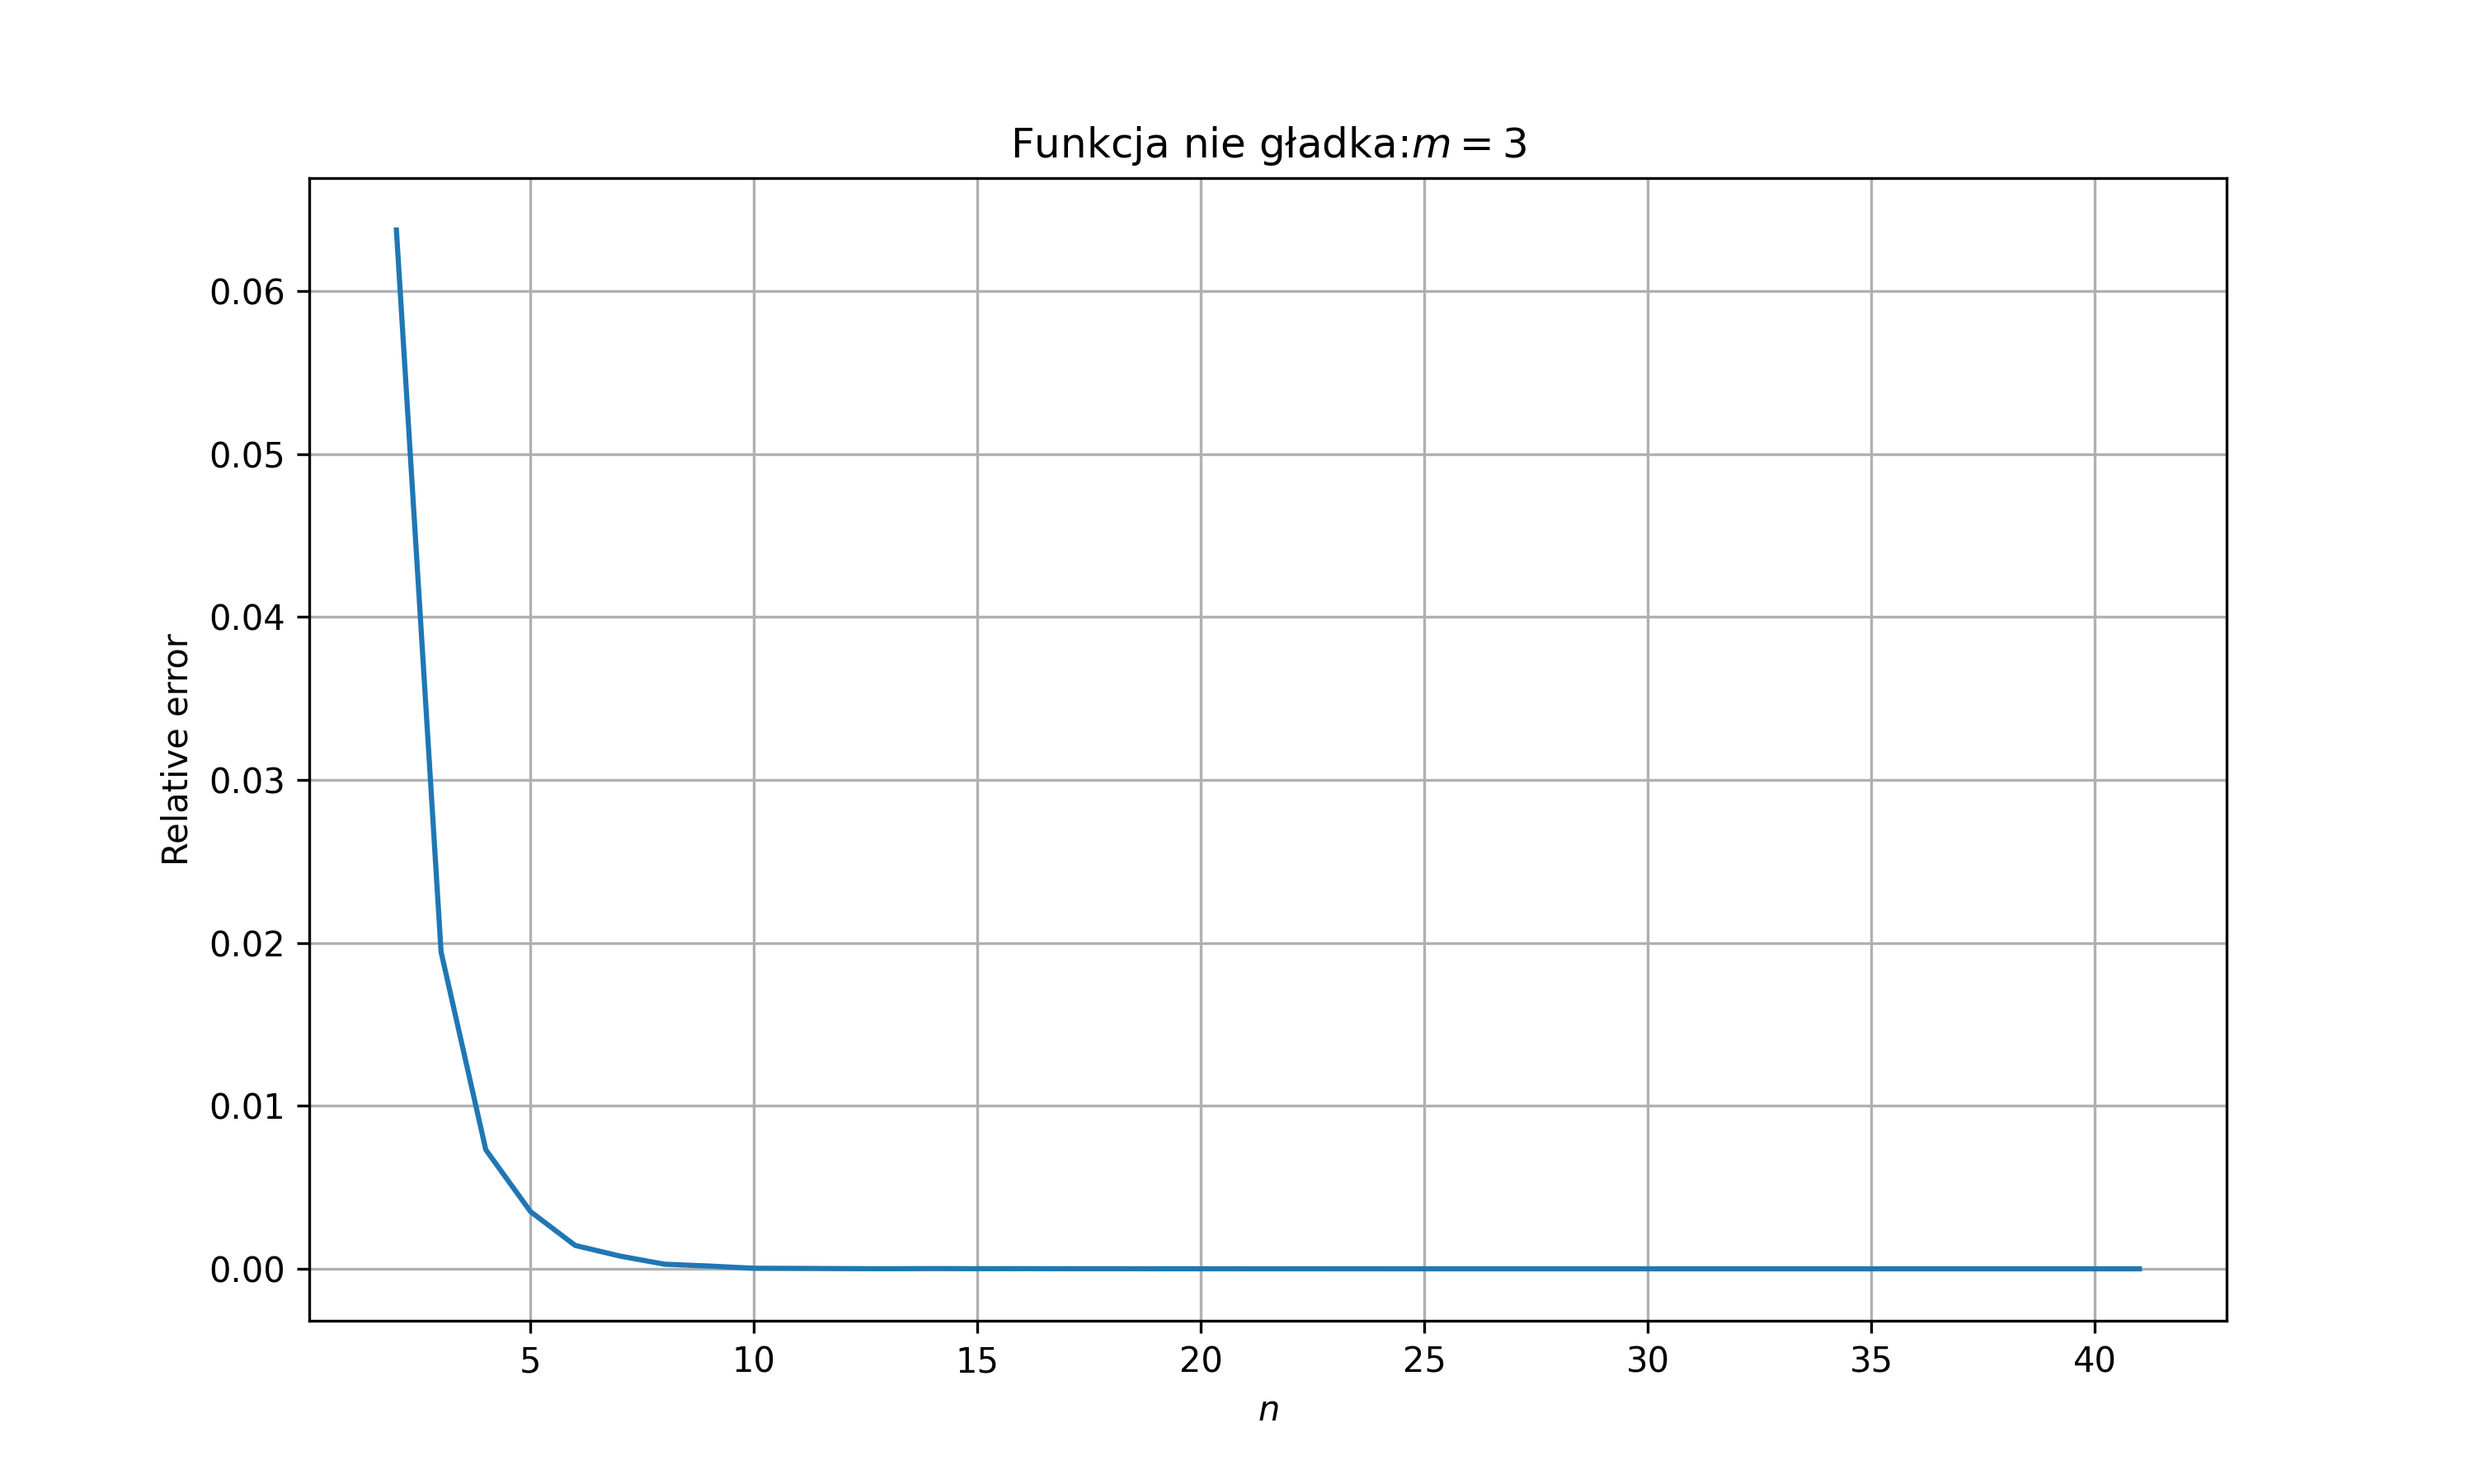
\includegraphics[width = \textwidth]{figures/task-1/nsmth_3.png}
\end{minipage}
\begin{minipage}{0.48\textwidth}
    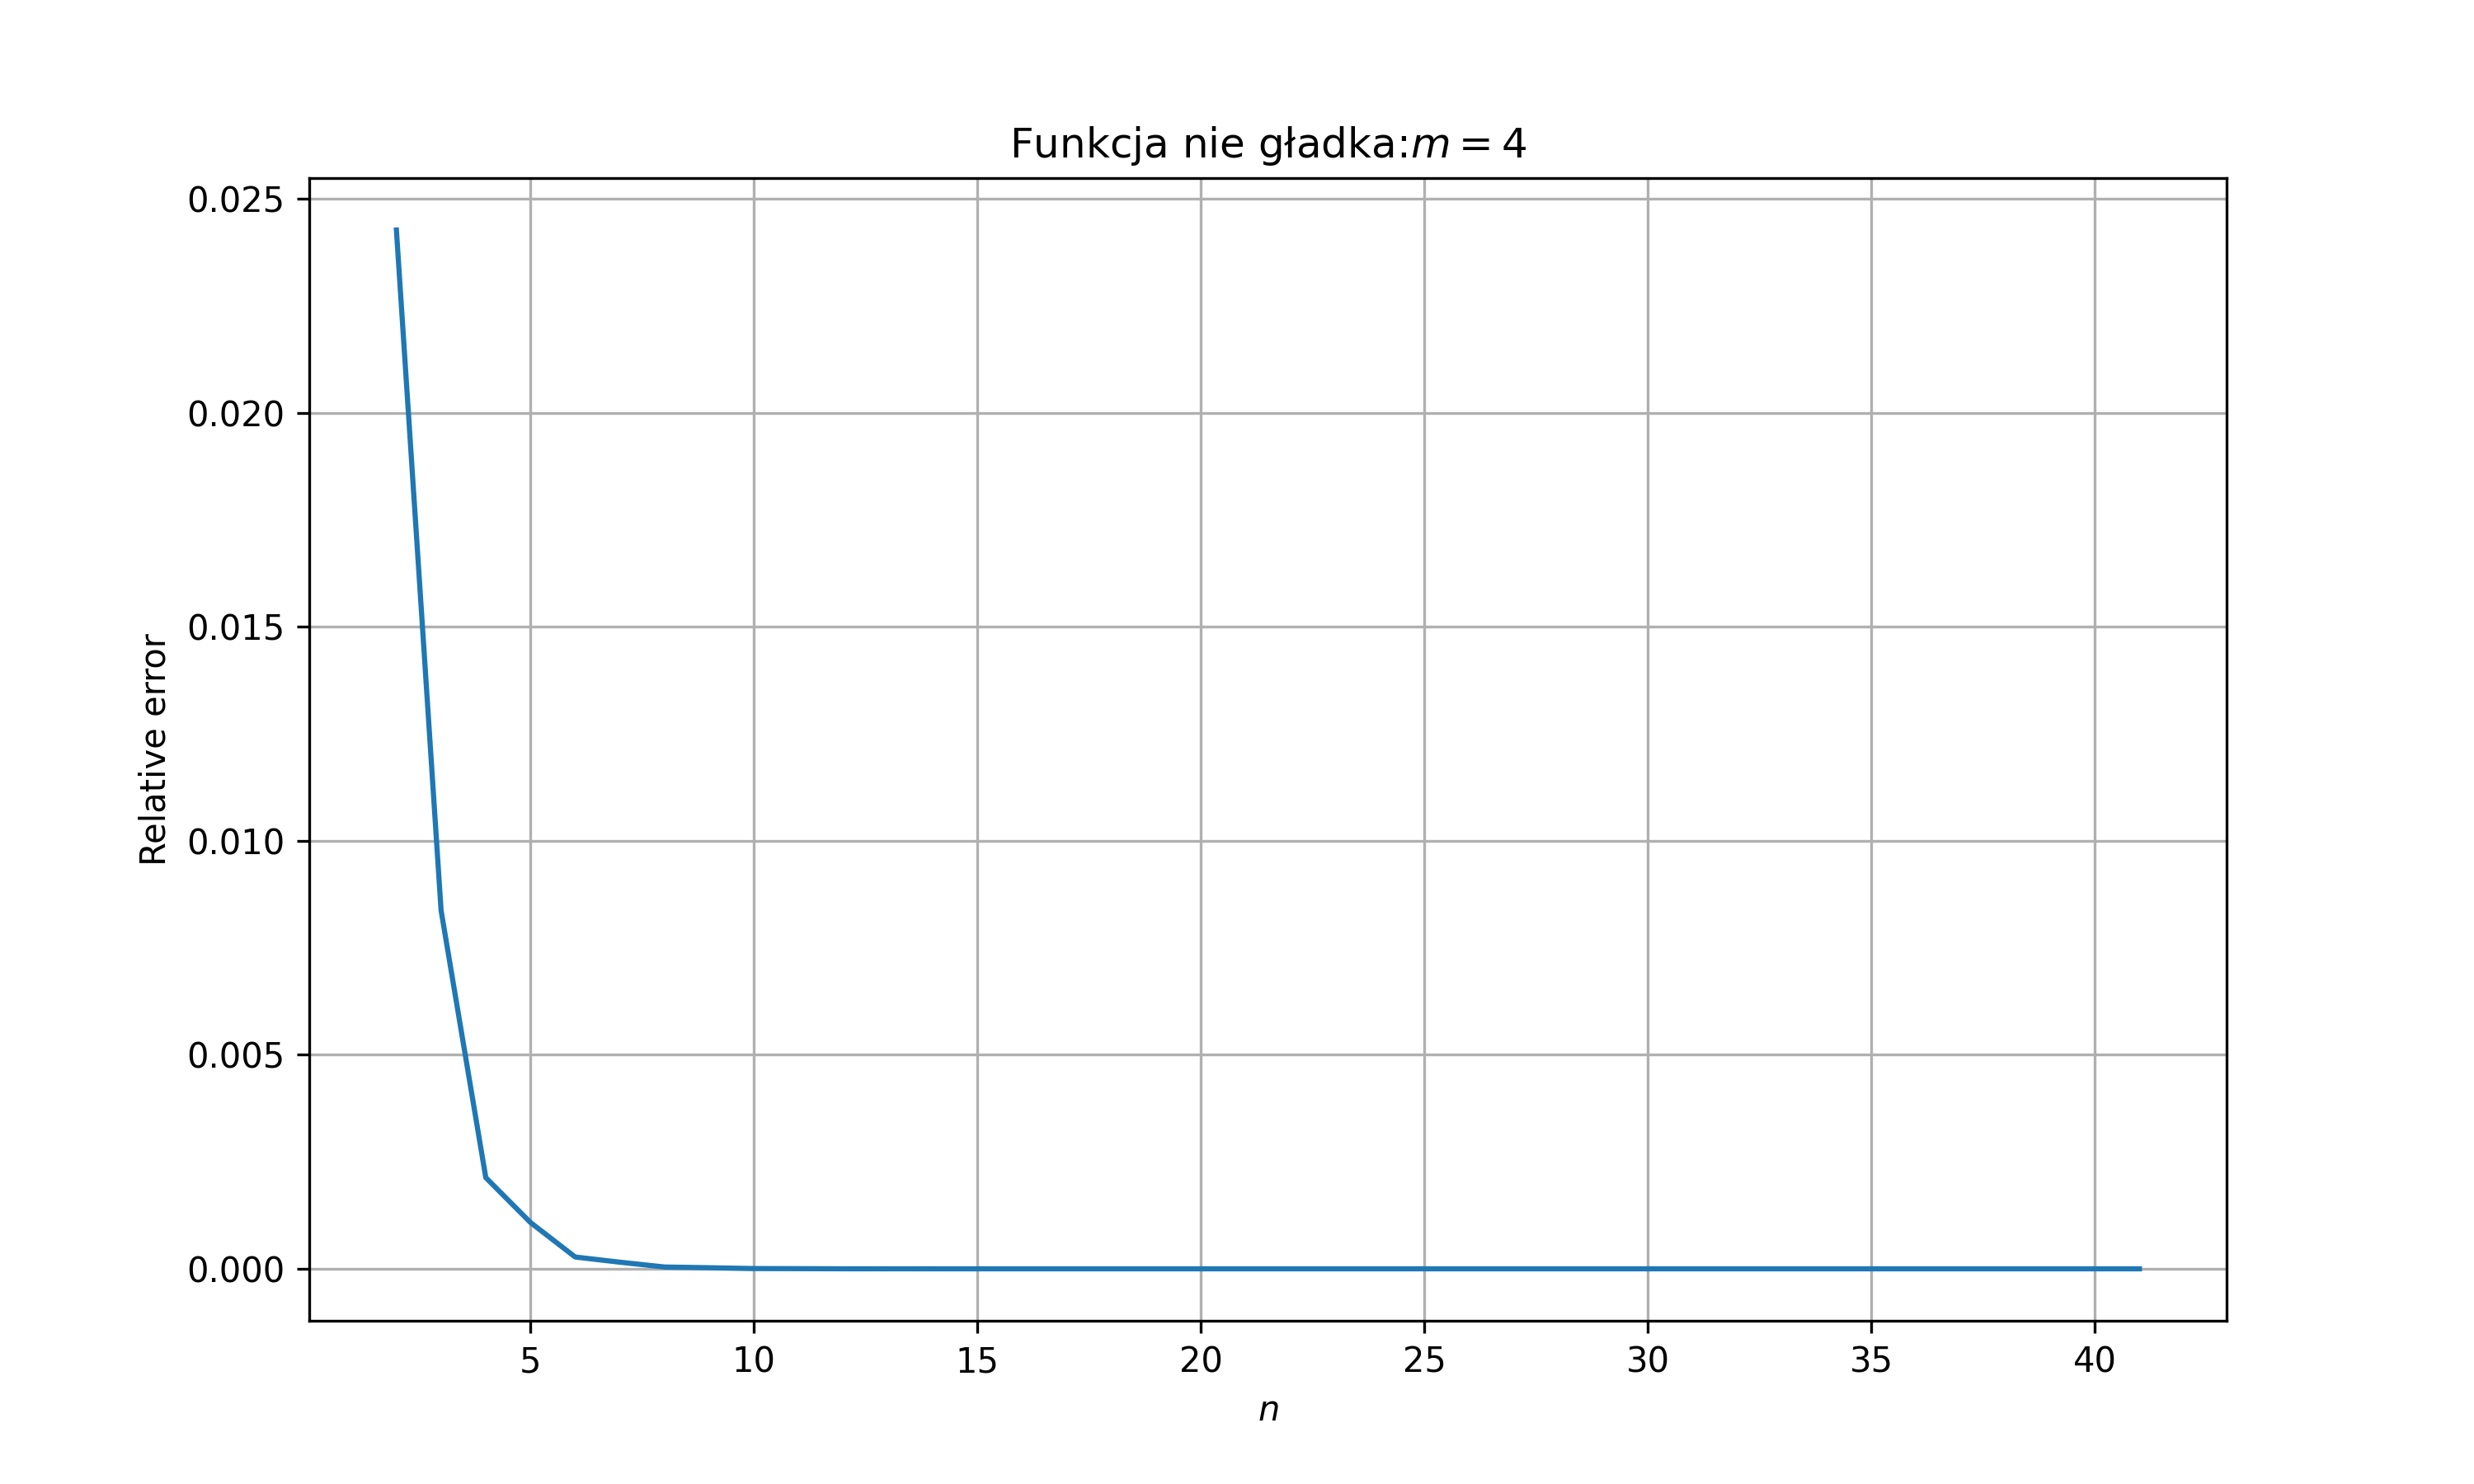
\includegraphics[width = \textwidth]{figures/task-1/nsmth_4.png}
\end{minipage}
Absolute error

}


\subsection{Conclusions and analysis}

The tests support the following conclusions:

\begin{itemize}
    \item Increasing \( m \), the formula order, drastically reduces the error. This is clearest for the function that is not uniformly continuous. Between 2 and 3, the error falls almost to zero, allowing accurate results quickly.
    \item High accuracy is attained quickly. However, too many intervals lead to the Runge phenomenon: the error starts increasing.
    \item The method could be optimized further. Compared with the \texttt{quad} method from \texttt{scipy.integrate}, it is the most accurate of the basic numerical methods.
\end{itemize}
